\documentclass[a4paper, 12pt]{article}

\usepackage[utf8]{inputenc}
\usepackage[spanish]{babel}
\usepackage{graphicx}
\usepackage{fancyhdr}
\usepackage{amssymb}
\usepackage{xcolor}
\definecolor{gray97}{gray}{.97}
\definecolor{gray75}{gray}{.75}
\definecolor{gray45}{gray}{.45}
\definecolor{deepblue}{rgb}{0,0,0.5}
\definecolor{deepred}{rgb}{0.6,0,0}
\definecolor{deepgreen}{rgb}{0,0.5,0}
\usepackage[hidelinks]{hyperref}
\usepackage[font=small, labelfont=bf]{caption} 
\usepackage{cite}


\usepackage{listings}
\lstset{ frame=Ltb,
framerule=0pt,
aboveskip=0.5cm,
framextopmargin=3pt,
framexbottommargin=3pt,
framexleftmargin=0.4cm,
framesep=0pt,
rulesep=.4pt,
backgroundcolor=\color{gray97},
rulesepcolor=\color{black},
%
stringstyle=\ttfamily,
showstringspaces = false,
basicstyle=\small\ttfamily,
commentstyle=\color{gray45},
keywordstyle=\bfseries\color{deepblue},
emphstyle=\ttb\color{deepred}, 
stringstyle=\color{deepgreen},
%
numbers=left,
numbersep=15pt,
numberstyle=\tiny,
numberfirstline = false,
breaklines=true,
}

%Para que listings reconozca los caracteres UTF-8
\lstset{literate=
  {á}{{\'a}}1 {é}{{\'e}}1 {í}{{\'i}}1 {ó}{{\'o}}1 {ú}{{\'u}}1
  {Á}{{\'A}}1 {É}{{\'E}}1 {Í}{{\'I}}1 {Ó}{{\'O}}1 {Ú}{{\'U}}1
  {à}{{\`a}}1 {è}{{\`e}}1 {ì}{{\`i}}1 {ò}{{\`o}}1 {ù}{{\`u}}1
  {À}{{\`A}}1 {È}{{\'E}}1 {Ì}{{\`I}}1 {Ò}{{\`O}}1 {Ù}{{\`U}}1
  {ä}{{\"a}}1 {ë}{{\"e}}1 {ï}{{\"i}}1 {ö}{{\"o}}1 {ü}{{\"u}}1
  {Ä}{{\"A}}1 {Ë}{{\"E}}1 {Ï}{{\"I}}1 {Ö}{{\"O}}1 {Ü}{{\"U}}1
  {â}{{\^a}}1 {ê}{{\^e}}1 {î}{{\^i}}1 {ô}{{\^o}}1 {û}{{\^u}}1
  {Â}{{\^A}}1 {Ê}{{\^E}}1 {Î}{{\^I}}1 {Ô}{{\^O}}1 {Û}{{\^U}}1
  {œ}{{\oe}}1 {Œ}{{\OE}}1 {æ}{{\ae}}1 {Æ}{{\AE}}1 {ß}{{\ss}}1
  {ű}{{\H{u}}}1 {Ű}{{\H{U}}}1 {ő}{{\H{o}}}1 {Ő}{{\H{O}}}1
  {ç}{{\c c}}1 {Ç}{{\c C}}1 {ø}{{\o}}1 {å}{{\r a}}1 {Å}{{\r A}}1
  {€}{{\euro}}1 {£}{{\pounds}}1 {«}{{\guillemotleft}}1
  {»}{{\guillemotright}}1 {ñ}{{\~n}}1 {Ñ}{{\~N}}1 {¿}{{?`}}1
}

% minimizar fragmentado de listados
\lstnewenvironment{listing}[1][]
{\lstset{#1}\pagebreak[0]}{\pagebreak[0]}

\lstdefinestyle{consola}
{basicstyle=\scriptsize\bf\ttfamily,
backgroundcolor=\color{gray75},
}

\lstdefinestyle{python}
{language=Python,
}



\topmargin=-1cm
\oddsidemargin=0cm
\textheight=24cm
\textwidth=17cm



\begin{document}

\renewcommand{\tablename}{Tabla}
\renewcommand{\refname}{Bibliografía}



\begin{titlepage}

\begin{minipage}{2.6cm}

\includegraphics[width=\textwidth]{fceia.pdf}
\end{minipage}
\hfill
%
\begin{minipage}{6cm}
\begin{center}
\normalsize{Universidad Nacional de Rosario\\
Facultad de Ciencias Exactas,\\
Ingeniería y Agrimensura\\
Departamento de Física -- ECEN\\}
\end{center}
\end{minipage}
\hspace{0.5cm}
\hfill
\begin{minipage}{2.6cm}

\includegraphics[width=\textwidth]{unr.pdf}
\end{minipage}


\vspace{0.5cm}

\begin{center}
\normalsize{\sc Física Computacional}\\
\vspace{0.5cm}
\Large{\bf Desarrollo del software PyReduc para reducción de imágenes astronómicas}\\


\vspace{5cm}

\normalsize
Carlos Mauricio Silva\\

\vspace*{0.5cm}
\small{\today}

\vspace*{3cm}

\begin{abstract}
  En este trabajo se presenta el desarrollo del software PyReduc, cuyo objetivo es reducir y apilar imágenes astronómicas en formato FITS. Se comentan los fundamentos de la reducción de imágenes y se explican las funciones principales del programa. Se comprueba el funcionamiento del software y se verifica que utilizando PyReduc para reducir y apilar imágenes astronómicas resulta en una mejora de la relación señal/ruido (SNR) de las imágenes.
\end{abstract}

\vspace{5cm}

\normalsize

\end{center}
\end{titlepage}


\pagestyle{fancy}
\lhead{\scriptsize{Desarrollo del software PyReduc}}
\rhead{\scriptsize{C. M. Silva}}
\lfoot{\scriptsize{Física Computacional}}
\cfoot{\scriptsize{Agosto de 2018}}
\rfoot{\scriptsize{Página \thepage}}
\renewcommand{\footrulewidth}{0.6pt}

\tableofcontents
\newpage

\section{Introducción teórica}
\subsection{Motivación}
Si hay una ciencia en la que cualquier ciudadano sin formación académica de grado puede hacer una contribución con un mínimo de equipamiento, esta es la Astronomía. Con la popularización de las cámaras ``DSLR'' (cámara digital réflex de una sola lente), cualquier persona con un poco de tiempo puede aprender laa técnicaa de astrometría y fotometría. Organizaciones como la Unión Astronómica Internacional (IAU) o la Asociación Americana de Observadores de Estrellas Variables (AAVSO) reciben las contribuciones de los observadores amateurs de todo el mundo, a quienes a través de diversas campañas se les ha comenzado a llamar ``científicos ciudadanos'' \cite{aavso}.


Si bien en Internet se puede encontrar software gratuito y de  alta calidad para realizar toda la tarea de procesado de imágenes astronómicas, estos están pensados principalmente para procesamientos artísticos o no están lo suficientemente automatizados para cumplir todas las tareas de preprocesado requeridas para poder reportar información con valor científico.

El objetivo de este trabajo es describir el funcionamiento del software \textbf{PyReduc}, desarrollado bajo las siguientes directivas:
\begin{itemize}
\item Cumplir con las libertades del Software Libre \cite{fsf}.
\item Constituir un conjunto de subrutinas  apto para realizar la reducción de imágenes, es decir el preprocesado necesario para obtener imágenes listas para realizar mediciones fotométricas sobre ellas.
\item Que el proceso de reducción sea, en la medida de lo posible, automático.
\item Que maneje el formato FITS, un formato de archivos estándar en investigación astronómica a nivel mundial. 
\item Que esté programado en un lenguaje de programación moderno, bien documentado y con librerías científicas de comprobada utilidad, como lo es el lenguaje Python.
\end{itemize}

\subsection{Algunos conceptos: Fotometría DSLR}
El objetivo de la fotometría es medir la intensidad de la luz que nos llega de los objetos celestes. Por ejemplo, en el caso de una estrella variable, esta información se hace relevante cuando se quiere obtener información sobre la evolución de la estrella en estudio.

El término ``DSLR''  se refiere a una clase genérica de cámaras
que es adecuada para llevar a cabo observaciones fotométricas. Recientemente, muchas cámaras
automáticas han comenzado a incorporar varias características requeridas para fotometría astronómica \cite{aavso}. 

En las cámaras DSLR, la imagen es capturada por un sensor electrónico de tipo CMOS (Semiconductor Complementario
de Oxido Metálico), sobre el que  se dispone un mosaico que filtra la luz en tres colores: rojo (R), verde (G) y azul (B). Estos mosaicos se conocen como mosaicos de Bayer.
Dependiendo del modelo y marca comercial de la cámara, estos mosaicos se pueden disponer en distintos órdenes. Así, por ejemplo, una la mayoría de las cámaras DSLR marca {\sf Canon} llevan un mosaico RGGB, lo que quiere decir que contiene dos celdas que detectan el verde, por cada celda de rojo y cada celda de azul. La estructura de estas cámaras escapa al objetivo de este trabajo, pero puede consultarse en la bibliografía \cite{aavso}.

El sensor en sí mismo está
hecho de un chip de silicio sobre el cual está grabado el circuito CMOS. El elemento sensible a los
fotones en cada píxel es un fotodiodo (o un sensor fotoeléctrico MOS). Tomemos, para orientarnos mejor, un único pixel en el sensor. Durante la exposición fotográfica, los fotones que van llegando al fotodiodo excitan electrones, los cuales se van almacenando en un capacitor originalmente descargado. Al final de la exposición, se lee la tensión en bornes del capacitor. Estas tensiones son muy pequeñas, por lo que para realizar la lectura se amplifican electrónicamente y luego un conversor analógico--digital (ADC) se encarga de convertirla en un número binario. En la fotometría DSLR se suele decir que este número está medido en ADU (Unidad Analógica--Digital). Este valor en ADU es el que se almacena en la matriz que conforma el archivo resultante.

Es interesante mencionar que, dado que los valores ADU registrados en la imagen son proporcionales a la cantidad de fotones que llegaron a cada pixel en cuestión, es un valor adecuado para tomar a la hora de hacer fotometría.



\subsection{El formato FITS}
Llamaremos a las imágenes de astros capturadas con fines científicos {\bf ``tomas científicas''} o {\bf ``lights''}. Las cámaras DSLR comerciales traen múltiples funciones. Entre ellas, hay algoritmos de balance de blancos, reducción de ruido, compensación de exposición, etcétera. La mayoría de estos algoritmos operan sobre los datos que capta el sensor y los modifican, por lo que es fundamental {\it no usarlos} para la fotometría. Todas las mejoras sobre las imágenes se deben hacer en perfecto control por parte del usuario. Es por ello que, al captar una toma científica, no se deben guardar en formato JPG. Al guardar en formato JPG, la imagen se convierte a un espacio de color llamado sRGB que es no lineal, y por lo tanto, no fotométrico.  El formato para almacenar tomas científicas sin pérdida de información es llamado
RAW. Un archivo RAW está formado, básicamente, por una matriz de números binarios. Cada elemento de la matriz contiene el valor ADU de cada pixel de la imagen. Además los archivos RAW conservan, en los {\it metadatos} de la imagen, información sobre la captura: marca y modelo de la cámara, sensibilidad ISO, velocidad de obturación, datos de la lente utilizada, si estuviera disponible, etcétera.

Dada la gran variedad de sensores CMOS y matrices Bayer, cada marca y modelo de cámara tiene su propio formato RAW. Para las diversas operaciones de medición astronómicas, se hace necesario tener un formato universal de imágenes. Es así que en el campo de la Astronomía y la Astrofísica se ha hecho extensivo el uso del formato FITS.

FITS es el acrónimo de {\it Flexible Image Transport System} (Sistema Flexible de Transporte de Imágenes). El formato FITS se empezó a desarrollar a fines de la década de 1970, con el uso de las primeras cámaras CCD, a los fines de compartir datos astronómicos entre instituciones que cooperaban entre sí. Una reseña histórica puede leerse en la bibliografía \cite{greisen}. Si bien la ``I'' en FITS significa ``Imágenes'', hoy en día sería más adecuada la palabra ``información'', ya que el formato FITS es mucho más que un formato de imagen. Como se establece en el sitio web de la Oficina de Soporte FITS de la NASA \cite{nasa}, en un archivo FITS se pueden guardar:

\begin{itemize}
  \item Arrays multidimensionales: Espectros 1D, imágenes 2D, Cubos de de datos de 3 o más dimensiones.
  \item Tablas que contengan filas y columnas de información (por ejemplo, coordenadas astrométricas).
  \item Una Cabecera con palabras clave (Header keywords) que provean información descriptiva sobre los datos.
\end{itemize}
  
  Un archivo FITS se divide, esencialmente en dos partes: La cabecera (header) y los datos (data).

\begin{figure}[!htb]
\begin{verbatim}
___________________________________________________________________
SIMPLE  =                    T / file does conform to FITS standard
BITPIX  =                   16 / number of bits per data pixel
NAXIS   =                    3 / number of data axes
NAXIS1  =                 5208 / length of data axis 1
NAXIS2  =                 3476 / length of data axis 2
NAXIS3  =                    3 / length of data axis 3
EXTEND  =                    T / FITS dataset may contain extensions
COMMENT   FITS (Flexible Image Transport System) format is defined in 'Astronomy
COMMENT   and Astrophysics', volume 376, page 359; bibcode: 2001A&A...376..359H
BZERO   =               32768. / offset data range to that of unsigned short
BSCALE  =                   1. / default scaling factor
INSTRUME= 'Canon EOS 700D'     / instrument name
DATE    = '2018-08-28T03:36:07' / UTC date that FITS file was created
DATE-OBS= '2018-04-14T01:36:33' / YYYY-MM-DDThh:mm:ss observation start, UT
XBINNING=                    1 / Camera binning mode
YBINNING=                    1 / Camera binning mode
EXPTIME =                  15. / Exposure time [s]
ISOSPEED=                1600. / ISO camera setting
BAYERPAT= 'RGGB    '           / Bayer color pattern
PROGRAM = 'Siril v0.9.9'       / Software that created this HDU
___________________________________________________________________
\end{verbatim}
\caption{Ejemplo de cabecera de un archivo FITS. Las palabras en mayúscula a la izquierda del signo {\tt =} son las palabras clave de la cabecera. El signo {\tt /} indica un comentario. \label{fig:header}}
\end{figure}

  
\paragraph{Cabecera FITS (Header)}
Es una sección del archivo FITS que contiene palabras clave que dan información sobre el archivo. Cuando se convierte una imagen RAW a un archivo FITS, es habitual que los {\it metadatos} de la imagen se guarden en la cabecera. También durante el procesado, esta información se va ampliando. Por tradición, la cabecera de los archivos FITS está codificada en caracteres de 7 bits ASCII.



Un ejemplo de cabecera FITS se muestra en la Figura~\ref{fig:header}.

No se presentará en este trabajo una descripción exhaustiva de las palabras claves obligatorias y opcionales que puede tener la cabecera de una archivo FITS. En cambio, se comentarán las más relevantes a los fines de este trabajo. Para más detalles, se puede consultar el manual del Estándar FITS de la Unión Astronómica Internacional \cite{fits}.

\begin{enumerate}
\item {\tt BITPIX}: Indica el número de bits por pixel (o elemento de matriz) en la sección de datos.
\item {\tt NAXIS}: Cantidad de ejes de datos. Se puede pensar como la dimensión de la matriz o el cubo de datos. En el ejemplo de la Figura~\ref{fig:header}, {\tt NAXIS1} y {\tt NAXIS2} corresponden a los dos ejes de la imagen, mientras que {\tt NAXIS3} corresponde a la cantidad de capas de color. Así podríamos decir que la imagen referenciada en el ejemplo tiene $5208 \times 3476$ pixeles y tres capas de color. La imagen de este ejemplo ya fue separada en los tres colores de los filtros del sensor. Las imágenes RAW que provienen de cámaras DSLR, deben ser separadas en colores de acuerdo con la organización del mosaico Bayer. Este proceso de descomposición se conoce como {\bf debayerizado} (debayering) o {\bf desmosaicado} (demosaicing). Si {\tt NAXIS} vale n, entonces deberán estar, necesariamente, las palabras claves {\tt NAXIS1}, {\tt NAXIS2}, ..., {\tt NAXISn}.
\item {\tt INSTRUME}: Indica marca y modelo del instrumento utilizado. Se obtiene, habitualmente, de los metadatos de la imagen RAW.
\item {\tt BAYERPAT}: Indica el patrón del mosaico Bayer de la cámara. No suele estar en los metadatos de la imagen RAW, así que al convertir el archivo a FITS se suministra esa información desde una base de datos de modelos de cámaras.
\item {\tt EXPTIME}: Es el tiempo de exposición de la imagen, medido en segundos. Equivale al tiempo que el obturador permanece abierto en una cámara convencional. En fotografía astronómica artística estos tiempos de exposición suelen ser de varias horas. A los fines de la fotometría, no es necesario tanto tiempo de exposición, fundamentalmente si se tiene en cuenta que la cámara tiene una respuesta lineal en un cierto rango de ADU. Cuando los tiempos de exposición son muy largos, puede suceder que el objeto de interés esté {\it sobreexpuesto}. En ese caso, el valor ADU registrado no será un valor proporcional a la cantidad de fotones captados por el sensor. Luego, para elegir el tiempo de exposición, un factor clave a tener en cuenta es la {\it curva de linealidad} del sensor.
\item {\tt ISOSPEED}: Es la configuración ISO en la que fue tomada la imagen. Muchas veces se dice que la configuración ISO se relaciona con la ``sensibilidad'' del sensor, pero en realidad la sensibilidad no cambia al cambiar el ajuste ISO. Lo que verdaderamente cambia con esta configuración es la {\bf ganancia} del sensor. La  ganancia se suele medir en electrones por ADU ($e^{-}$/ADU), y es una medida de la amplificación de la señal.
  Cuando un fotón llega al sensor, existe siempre la misma probabilidad de que este excite un electrón produciendo una señal. Esta respuesta a la excitación sería la sensibilidad del sensor. La ganancia, en cambio, está caracterizada por la amplificación de la señal producida. Configuraciones ISO más altas dan una ganancia más pequeña. Esto significa que para obtener una unidad ADU, a ISO más alto, se necesitará excitar menos electrones. Resumiendo, podemos decir que a mayor ISO, mayor amplificación de la señal, y menor ganancia. Un problema que surge al aumentar la configuración ISO es que también aumenta el ruido. Es por ello que, para fotografía astronómica no se usan las configuraciones ISO más altas. En fotografía astronómica artística, las configuraciones ISO suelen estar entre ISO 800 y 3200. En cambio, para las técnicas de fotometría, se busca que la ganancia del sensor sea cercana a 1 $e^{-}$/ADU. Como ejemplo, en la DSLR {\sf Canon EOS 700D}, esto se logra para ISO 200 o ISO 400. %En el Apéndice~\ref{ap:gain} se presentan gráficas de la ganancia del sensor para estas dos configuraciones.
\item {\tt DATE}: Es la fecha y hora de creación del archivo FITS.
\item {\tt DATE-OBS}: Es la fecha y hora en que se realizó la toma%\footnote{Como este informe, que fue escrito durante la toma de la FCEIA.}
  fotográfica, en {\it Tiempo Universal Coordinado}. Este valor se obtiene de los metadatos de la imagen, que a su vez se obtienen de la configuración de la cámara. Para esto, es importante que la hora de la cámara esté bien sincronizada con la hora oficial.

  Como decíamos, otras palabras claves son posibles, como la ubicación geográfica del observatorio, el nombre del observador, el nombre del objeto observado, sus coordenadas celestes, etcétera.
\end{enumerate}

\paragraph{Datos FITS}
Son los datos propiamente dichos, codificados en binario según la palabra clave {\tt BITPIX}, y ordenados en un arreglo de dimensiones indicadas por las palabras claves {\tt NAXIS1}, {\tt NAXIS2}, ..., {\tt NAXISn} de la cabecera. Con estos datos se trabajará en la reducción de imágenes y la fotometría.


\subsection{Reducción de imágenes: Tomas Dark, Bias y Flat}
\label{sec:tomas}
El proceso de reducción implica la eliminación de efectos instrumentales que estén presentes en los datos, ya sean de espectroscopía o de imagen directa. Es necesario llevar a cabo la reducción antes de poder realizar cualquier tipo de medida sobre nuestros datos. En este trabajo nos limitaremos a los efectos comúnmente presentes en las imágenes DSLR, pero esencialmente estos son los mismos efectos que se presentan en las imágenes con sensores CCD.

Podríamos decir que el mayor problema con el que hay que lidiar en la fotometría DSLR es con el ruido. Dado que en la fotometría necesitamos relevar la intensidad de la luz que proviene de las estrellas, necesitamos que el ruido sea lo sufientemente bajo para que no interfiera significativamente con las mediciones. Es por ello que el objetivo principal que se persigue con el proceso de reducción es incrementar la {\bf ``relación señal/ruido''} (SNR).

\subsubsection{Tomas Bias}
\label{sec:bias}
Al igual que en las tomas Dark, las tomas Bias se realizan con el objetivo tapado, y la misma configuración ISO que las tomas científicas, pero con la exposición más corta que proporcione la cámara (por ejemplo, 1/4000 s). Estas tomas contienen el ruido electrónico y de lectura propio del sensor. Este ruido está presente en todas las tomas, independientemente de la exposición y de la temperatura del sensor. Con el conjunto de tomas Bias se realiza un apilado promediando los valores de los pixeles homólogos de cada imagen, o bien tomando la mediana de dichos valores. Al hacer esto se crea un \textbf{``Master Bias''}.

\subsubsection{Tomas Dark}
Una de las correcciones que se pueden hacer a nuestras tomas científicas es la corrección por tomas Dark. Las tomas Dark se realizan con la misma configuración ISO que las tomas científicas y la misma exposición, pero ``en la oscuridad''. Para ello, se tapa el objetivo de la cámara o del telescopio y se dispara una serie de tomas, usualmente más de diez. Las tomas Dark, entonces, no contienen ``información'', pero contienen ruido térmico asociado con el sensor. Este ruido térmico es fuertemente dependiente de la temperatura y de la exposición. Así, para exposiciones menores a 30 s, pueden no ser necesarias estas tomas de calibración. Sin embargo, para exposiciones prolongadas, el sensor va aumentando su temperatura y el ruido térmico se hace más evidente. También la temperatura ambiente juega un rol fundamental en esta ecuación. Es por ello que las tomas Dark deben hacerse durante la misma sesión fotográfica, aunque eso quite tiempo de exposición para las tomas científicas.

\begin{figure}[!ht]
  \centering
  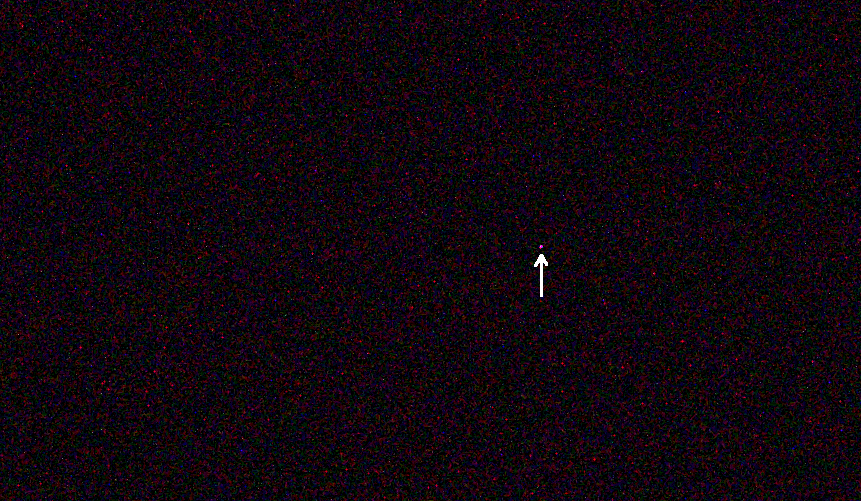
\includegraphics[width=0.75\textwidth]{img/dark.png}
  \caption{\label{fig:dark} Recorte y ampliación de una toma Dark realizada con una DSLR Canon EOS 700D en un telescopio Maksutov-Cassegrain de 102 mm f/12,7. La imagen RAW está debayerizada y el contraste está levemente realzado. La flecha blanca muestra un defecto que no vuelve a aparecer en el resto de imágenes Dark de la serie y se puede deber, por ejemplo, al efecto de rayos cósmicos impactando en el sensor. Si este efecto apareciera en toda la serie de imágenes, entonces podríamos decir que es un defecto de lectura del sensor, conocido como ``hot pixel''.}
\end{figure}

Con el conjunto de tomas Dark, usualmente se hace un apilado promediando los valores de los pixeles homólogos de cada imagen, o bien tomando la mediana de dichos valores.  Sin embargo, como se decía en la sección \ref{sec:bias}, estas tomas también tendrán ruido electrónico y de lectura. Para quitar esta contribución, se le puede restar a cada toma Dark un Master Bias. Este último proceso es especialmente importante si las tomas Dark no tienen el mismo tiempo de exposición que las tomas científicas. Finalmente se deben apilar las imágenes Dark corregidas utilizando el promedio o la mediana de los pixeles, obteniendo así una imagen que se llama \textbf{``Dark-current''}. Antes de restar la imagen Dark-current a las tomas científicas, se las debe escalar por un factor igual al cociente entre el tiempo de exposición de las tomas científicas y de las tomas Dark.

\subsubsection{Tomas Flat}
Los telescopios y las lentes comerciales usualmente no iluminan el sensor en forma homogénea. Habitualmente, la luz se distribuye en mayor cantidad en el centro del sensor que en los bordes. Este defecto en las imágenes se llama viñeteo. Más aún, las superficies ópticas de los telescopios y lentes suelen acumular polvo (y el sensor de la cámara también). A esto hay que agregarle que el propio sensor no tiene la misma respuesta en todos sus pixeles a un mismo estímulo lumínico. 
La Figura~\ref{fig:flat} muestra una toma flat individual con el contraste realzado para mostrar algunos defectos que se pueden presentar en una imagen. A diferencia de los ruidos térmico y de lectura, que eran contribuciones aditivas a las tomas científicas, estos defectos son de carácter multiplicativo. Para corregir estos defectos, se debe dividir a las tomas científicas por un {\bf ``Master Flat''}.

\begin{figure}[!ht]
  \centering
  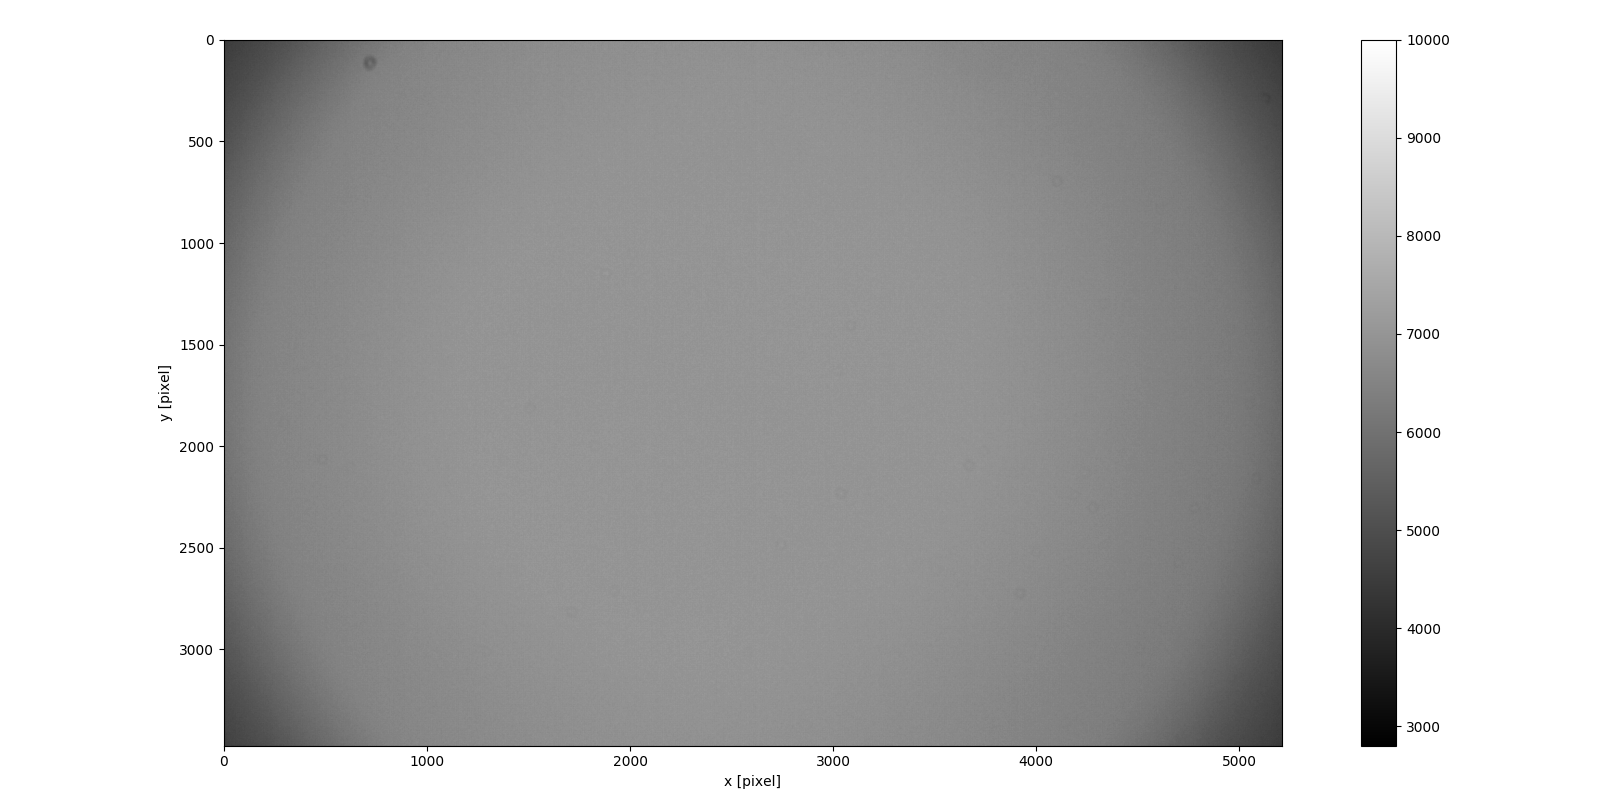
\includegraphics[width=\textwidth]{img/flatx.png}
  \caption{\label{fig:flat} Toma Flat realizada con una DSLR Canon EOS 700D en un telescopio Maksutov-Cassegrain de 102 mm f/12,7.  Los números en los ejes indican coordenadas en pixeles. La barra lateral indica los niveles de brillo del histograma. Se muestra solo el canal verde de la imagen. Se observa en las esquinas de la imagen el efecto de viñeteo debido a una iluminación no homogénea del sensor. También arriba a la izquierda de la imagen se ve una mancha circular que se debe a un resto de polvo en el tren óptico del instrumento.}
\end{figure}

Para fabricar un Master Flat, se deben sacar varias tomas apuntando el objetivo a una superficie uniformemente iluminada por luz blanca, sin llegar a saturar el sensor. Una manera simple y moderna de hacerlo es apuntar el telescopio a un monitor LCD (sin remover la cámara de su posición en el tubo). Las cámaras DSLR comerciales tienen un modo AV en el que la cámara calcula el tiempo de exposición automáticamente. Este modo usualmente proporciona Flats muy adecuados. La configuración ISO en el caso de las tomas Flats debe ser menor o igual a la de las tomas científicas.

Una vez que se tienen las tomas Flat, se les debe quitar el ruido de lectura y térmico restándole los Master Bias y Dark-current (escalado con el tiempo de exposición de los Flats). Luego se las apila utilizando la mediana, siendo el resultado obtenido el Master Flat. Antes de dividir las tomas científicas por el Master Flat, se le debe realizar un escalado o normalización, ya que es posible que los niveles de iluminación sean diferentes para cada imagen. Una opción posible sería darle peso a cada imagen Flat usando su mediana. Se promedian todas las imagenes Flats utilizando esos pesos, y se divide esta imagen resultante por el promedio de todos sus pixeles. La imagen Master Flat resultante está, entonces, reducida y normalizada.


Las correcciones explicadas en toda esta sección \ref{sec:tomas} se pueden condensar en la fórmula~(\ref{eq:reduc}).


\begin{equation}
  \mbox{Científicas}_{reducidas} = \frac{\mbox{Científicas}_{raw} - \mbox{Master~Bias}-\mbox{Dark~current}_{escalada}}{\mbox{Master~Flat}_{reducida,~normalizada}}
  \label{eq:reduc}
\end{equation}

 Esta fórmula de reducción de imágenes científicas que se utiliza aquí fue tomada del curso
 ``Introduction to Astronomical Image Analysis'' de  Matthew Craig, Juan Cabanela y Linda Winkler \cite{craig}.

Una vez que la serie de imágenes científicas fueron reducidas, se puede proceder a realizar las mediciones fotométricas. Sin embargo, si se busca realizar una medición precisa de un objeto muy débil, se puede aumentar aún más la SNR. Esto se logra realizando un apilado (en inglés \textit{stacking}) de un conjunto de tomas científicas reducidas de la misma región del cielo. Para este apilado existen diferentes algoritmos. El más sencillo consiste en promediar los pixeles homólogos de cada imagen, como se hacía con las tomas de calibración. Otros algoritmos consisten en realizar ese promedio, pero descartando valores extremos o reemplazándolos por valores que  se encuentren dentro de ciertos percentiles.

Como último detalle, puede que la serie de imágenes no estén perfectamente alineadas, por ejemplo, porque el seguimiento del telescopio utilizado no es perfecto. Es por ello que muchas veces se hace necesario hacer una alineación, llevando todas las imágenes de la serie a un mismo sistema de coordenadas mediante traslaciones, rotaciones y, en casos más raros en que se usen distintas lentes, cambios de tamaño. Este proceso se llama {\bf ``Registro de imágenes''} \cite{brown}.

\section{Metodología}
Para desarrollar el programa PyReduc se ha utilizado el lenguaje de programación Python 3. Este lenguaje de alto nivel, interpretado y orientado a objetos, posee una gran variedad de librerías científicas. Entre ellas, la librería \texttt{NumPy} es fundamental para trabajar con vectores, matrices y arreglos N-dimensionales. Integrado dentro de la gran librería \texttt{SciPy}, \texttt{Matplotlib} permite graficar \textit{al vuelo} funciones, datos o imágenes de mapas de bits. Por otro lado, la librería \texttt{Astropy} es un esfuerzo comunitario por desarrollar todo un ecosistema de paquetes astronómicos que sean interoperables en lenguaje Python \cite{astropy}. Entre ellos, el módulo \texttt{astropy.io.fits} permite manejar ficheros FITS. Está basado en el módulo \texttt{PyFITS} desarrollado por el Space Telescope Science Institute. El proyecto \texttt{PyFITS} se unió a \texttt{Astropy} como parte de estos esfuerzos de desarrollar una gran librería--ecosistema de paquetes astronómicos.

Dado que PyReduc está pensado para realizar reducciones que luego se utilizarán para fotometrías, el programa está pensado para procesar  imágenes FITS monocromáticas. En el caso de imágenes RAW DSLR, será necesario, antes de utilizar PyReduc, realizar el debayerizado y extraer un canal con algún software externo. Una posibilidad sería utilizar el script de M. Emre Aydin \texttt{cr2fits} \cite{aydin}, que permite extraer un solo canal de una imagen RAW y la convierte en FITS, transcribiendo todos los metadatos necesarios.

Las imágenes FITS deben estar en un directorio llamado ``\texttt{\~/pyreduc/FITS/}'',  donde ``\texttt{\~}'' representa el directorio \texttt{HOME}. Los prefijos de los archivos deben seguir las siguientes reglas:
\begin{itemize}
\item[--]  FLATS: ``\texttt{flat*}''
\item[--]  DARKS: ``\texttt{dark*}''
\item[--]  BIAS: ``\texttt{bias*}''
\end{itemize}
donde ``*'' significa ``cualquier cosa a partir de aquí''.
El prefijo de las tomas científicas se ingresa por teclado.

Por ejemplo:\\

 En la carpeta ``\texttt{\~/pyreduc/FITS/}'' se tienen los archivos:
\begin{verbatim}
  - bias001.fit, bias002.fit, bias003.fit bias004.fit,...
  - darkA.fit, darkB.fit, darkC.fit,...
  - flat_0001.fit,..., flat_0005.fit,..., flat_0011.fit
  - RCnc_001.fit, RCnc_002.fit, RCnc_003.fit,...,
\end{verbatim}
 entonces las tomas de calibración tienen el nombre correcto. Cuando el programa pida el prefijo de las tomas científicas,
se deberá ingresar por teclado:
\begin{verbatim}
	RCnc
\end{verbatim}





Una vez que todos los archivos FITS de tomas científicas, Flats, Dark y Bias están dispuestas en una carpeta FITS dentro del directorio \texttt{\~/pyreduc/FITS/}, PyReduc las copia, utilizando la librería \texttt{shutil}, a un nuevo directorio llamado ``\texttt{\~/pyreduc/procesado/}'', en el que se realizará el proceso de reducción.

Utilizando la librería \texttt{glob}, se arman 4 objetos de tipo {\em lista} de Python 3, que contendrán las tomas científicas, dark, bias y flat. Luego, empleando la librería {\tt astropy.io.fits} se leen las cabeceras de estos archivos y se imprimen por pantalla los nombres de archivos junto con la resolución en pixeles de cada imágen y el tiempo de exposición.

La cantidad de archivos de cada lista se guarda en una variable distinta. Además se guardan en sendas variables el tiempo de exposición de cada tipo de toma. En este punto, hay que destacar que en PyReduc suponemos que todas las tomas de un mismo tipo tienen el mismo tiempo de exposición, por lo que puede que alguna parte del proceso no se cumpla si esta suposición no es verdadera.

Una vez hecho esto, comienza el proceso de reducción propiamente dicho. Este proceso está basado en un trabajo de Ricardo Gil-Hutton \cite{gil-hutton}. Este tutorial estaba basado en la librería \texttt{PyFits},
pero en PyReduc se ha  reemplazado por {\tt astropy.io.fits}.


 Para realizar el procesado de Bias se creó una función llamada \texttt{mediana\_calib}, cuyos argumentos son la lista\footnote{Aquí {\it lista} se usa en el sentido del objeto Python de tipo lista.} de imágenes a procesar y la cantidad de estas imágenes. La función creada ejecuta el procedimiento descripto a continuación:
 \begin{enumerate}
 \item Primero se arma un arreglo tridimensional en donde se ponen todas las imágenes Bias secuencialmente, de manera que el elemento $a_{ijk}$ del arreglo es el pixel de coordenadas $(j,k)$ de la {\it i-ésima} imagen Bias.
 \item Luego se ordenan los pixeles de la secuencia de imágenes de menor a mayor a lo largo del primer eje. Para clarificar esto, se toman los pixeles de coordenadas fijas $(j,k)$ de cada imagen de la secuencia y se los ordena de mayor a menor en el arreglo tridimensional. Así, la matriz que se obtendría de fijar el índice $i=0$ estaría formada por los pixeles de menor valor de todas las imágenes\footnote{A diferencia del lenguaje FORTRAN, en el lenguaje Python los índices de los arreglos comienzan en 0.}. Este ordenamiento se realiza con la función \texttt{sort} de la librería \texttt{NumPy}.
 \item Finalmente se calcula la mediana de todos los pixeles de coordenadas $(i,j)$ fijas, pero descartando los pixeles de valor más alto. La razón de este descarte es eliminar posibles defectos como el que se ve en la Figura~\ref{fig:dark}. Este cálculo de la mediana se realiza con la función \texttt{median} de la librería \texttt{NumPy}.
 \end{enumerate}

 

 La imagen así obtenida constituye el Master Bias, el cual se guarda en memoria, en un array de \texttt{NumPy} de nombre \texttt{stbias}. A continuación, se sigue con el procesado de tomas Dark. Lo primero que se hace es restarle a todas las tomas Dark el Master Bias, formando así tomas pre-Dark-current. Para este fin, se creó una función llamada \texttt{resta\_master} cuyos argumentos son la lista de imágenes a procesar y la imagen Master que se les va a restar. Cabe destacar que esta función sobreescribe las imágenes de la lista que se le pasa como argumento, reemplazándolas por las nuevas imágenes pre-Dark-current.

 Una vez que se tienen las imágenes pre-Dark-current, se utiliza la función \texttt{mediana\_calib} para apilar estas tomas utilizando la mediana y descartando los valores de los pixeles más altos. La imagen así obtenida constituye la toma Dark-current buscada y se guarda en memoria en el arreglo \texttt{stdark}

 Para realizar la calibración utilizando la fórmula (\ref{eq:reduc}), primero se crea una imagen que es la suma de la Master Dark y de la Dark-current escalado con el tiempo de exposición de las tomas científicas. Esta imagen, que en el programa se guarda en memoria en el arreglo de \texttt{NumPy} \texttt{master\_stack}, obedece a la siguiente expresión:
 \begin{equation}
   \label{eq:master}
   \mbox{master\_stack} = \mbox{Master Bias} + \frac{exp_{dark}}{exp_{lights}}\ \mbox{Dark-current}
 \end{equation}
 en donde $exp_{dark}$ es el tiempo de exposición de las tomas dark y $exp_{lights}$ es el tiempo de exposición de las tomas científicas. Aquí es importante mencionar que en este programa estamos suponiendo que todas las tomas Dark tienen el mismo tiempo de exposición entre sí, y que lo mismo ocurre con las tomas científicas.

 Una vez construida la toma de calibración \texttt{master\_stack}, se la resta a todas las tomas científicas, recurriendo nuevamente a la función \texttt{resta\_master}.

 A continuación, se calibran todas las tomas Flat con una nueva imagen \texttt{master\_stack}, construida utilizando la expresión (\ref{eq:master}), pero reemplazando el tiempo de exposición de las tomas científicas por el de las tomas Flat.

 Para apilar las tomas Flat ya calibradas, el proceso es ligeramente diferente al de los Dark-current y los Bias, ya que estas tomas usan iluminación artificial. Como es posible que los niveles de iluminación de cada toma sean diferentes, se le da peso a cada imagen con su mediana. Se crea un arreglo tridimensional de imágenes Flat tal como se hacía para los Bias y los Dark, pero con dicho peso. Luego se calcula una nueva imagen promediando los pixeles homólogos de cada imagen y despreciando los valores más altos, pero se normaliza el resultado con la suma de las medianas de cada imagen. Así se obtiene una imagen Master Flat de buena relación señal/ruido, que se puede usar para hacer la corrección de las
imágenes científicas. Esto se realiza dividiendo por el Master Flat y reescalando con su media para no modificar el valor medio
de cada imagen.

De esta manera, la calibración basada en la fórmula de reducción (\ref{eq:reduc}) queda completada.

Antes de proceder al apilado de las imágenes, es necesario alinearlas. Para este proceso se ha escrito un módulo llamado \texttt{registrado} que es en realidad un script que utiliza las herramientas de \texttt{astroalign} para alinear las imágenes previamente calibradas. Astroalign es un paquete que alinea dos imágenes astronómicas buscando asterismos de tres puntos (tres estrellas) en común entre las dos imágenes, y
realizando una transformación afín entre ellas. El autor del paquete astroalign es Martin Beroiz \cite{astroalign}. Dado que el proceso de alineación o registro de imágenes está fuera del alcance de este informe, solo se mencionará que la función \texttt{registra\_lista}, dentro del módulo registrado, recibe como argumento la lista de imágenes a registrar y sobreescribe las imágenes de esa lista con nuevas versiones a las que se le aplicaron las transformaciones necesarias para un posterior apilado exitoso.

Una vez finalizado el alineado, el programa está listo para realizar el apilado de las tomas científicas. Para ello, se escribió un módulo llamado \texttt{apilado}, que tiene dos opciones a elegir por el usuario:
\begin{enumerate}
\item Apilado realizando el promedio de todos los pixeles homólogos de cada imagen.
\item Apilado con descarte de valores extremos (``pixel rejection'').
\end{enumerate}

Para ambas opciones, se construye un arreglo tridimensional con todas las tomas científicas reducidas, igual que se hacía para las tomas de calibración. Luego, según la opción elegida por el usuario, este arreglo se pasa como argumento a una de las dos funciones escritas para el apilado.

Para la primera opción, la función \texttt{no\_rejection} simplemente toma todos los pixeles homólogos de todas las tomas científicas ya calibradas y alineadas y realiza el promedio. El resultado es una nueva matriz de nombre de variable \texttt{stack} que se devuelve a la subrutina principal.

La segunda opción, que fue escrita desde cero para PyReduc, es algo más compleja. La idea del algoritmo contenido en la función \texttt{pixel\_rejection} es tomar los pixeles homólogos de cada imagen y promediarlos, pero rechazando aquellos que se aparten más de dos desviaciones estándar del promedio. El algoritmo se muestra en el Apéndice \ref{sec:apilado}.

Finalizado el apilado, la imagen resultante se guarda en el archivo \texttt{stacking.fit}. Luego, el programa da la opción de visualizar dicha imagen. Para este fin, se ha escrito el módulo \texttt{visualizacion.py} que utiliza la librería {\tt matplotlib} para representar la imagen en pantalla. En este punto es necesario mencionar que toda imagen se puede caracterizar con un histograma que de cuenta de la frecuencia con la que aparecen los diferentes valores de pixeles en la imagen. Dado que las imágenes FIT resultantes habitualmente tienen una cantidad de niveles de brillo muy extensa, para poder apreciar los detalles de la imagen se hace necesario retocar el histograma de la imagen de alguna manera. Para ello, el módulo de visualización consta de tres opciones:
\begin{enumerate}
\item La opción manual, que le muestra al usuario el histograma para que este elija un valor máximo y un mínimo entre los cuales recortar. Así, el usuario ajusta el histograma entre estos dos niveles de brillo. El usuario también puede escoger si al mostrarse la imagen se usa una interpolación bilineal para suavizarla o no.
\item El reescalado automático del histograma entre los percentiles 2 y 98. Para este reescalado automático se utiliza la función {\tt exposure.rescale\_intensity} de la librería {\tt skimage}. Luego, en la representación de la imagen se utiliza una interpolación bilineal.
\item Una ecualización automática del histograma. En la representación se utiliza una interpolación bilineal.
\end{enumerate}

Para la última opción, se ha escrito para PyReduc un último módulo, {\tt ecualizado.py} que es una implementación en lenguaje Python de un método muy difundido de ecualización de histogramas para el procesamiento digital de imágenes. La implementación se hizo a partir del algoritmo explicado en el libro ``Image Processing in C'' de Dwayne Phillips \cite{phillips}. El método de ecualización {\it mapea} un histograma que presenta picos notorios en otro más {\it aplanado} o {\it ecualizado}. Aplanar el histograma hace que los pixeles oscuros aparezcan a la vista más oscuros y que los pixeles claros aparezcan a la vista más claros. En el Apéndice \ref{sec:ecualizado} se explica un poco más del método de ecualizado y se lista el código implementado.


Cabe destacar que las tres opciones de visualización trabajan en memoria RAM, por lo que ninguna de ellas altera realmente los datos de la imagen. En la ventana de visualización, el usuario puede encontrar un botón para guardar la imagen que está visualizando en un archivo con algún formato de mapa de bits tradicional, como el formato PNG. Al cerrar la ventana de visualización, las modificaciones al histograma se pierden.

Vale la pena mencionar, que este módulo de visualización se puede ejecutar independientemente del resto del programa PyReduc, siempre y cuando la imagen que se quiera visualizar tenga formato FITS y nombre de archivo \texttt{stacking.fit}.

 
\section{Resultados}
Para probar el programa PyReduc se utilizó una serie de imágenes de la nebulosa Messier 8 (M8), más conocida como Nebulosa Laguna. La secuencia de imágenes se realizó con una cámara {\sf Canon EOS 700D} a foco primario en un telescopio Maksutov-Cassegrain de 102 mm de diámetro y relación focal f/12,7. Como se mostró en la Figura~\ref{fig:flat}, este dispositivo presenta un viñeteado significativo, que vuelve imprescindibles las tomas de calibración Flat. Se emplearon 9 tomas científicas de 30 s de exposición a ISO 3200\footnote{Este valor de ISO es bastante elevado para realizar fotometría, ya que se aleja mucho de la ganancia de $1 e^{-}$/ADU del sensor, pero es útil para probar las funciones de PyReduc, por la cantidad de información que es capaz de muestrear}. Para la calibración se realizaron 20 tomas Bias de $0.00025$ s de exposición, 10 Dark de 30 s de exposición y 15 Flat de 0,25 s de exposición. Previamente a la utilización de PyReduc, se extrajo de todas las imágenes RAW el canal verde y se creó así una nueva secuencia de imágenes FITS, utilizando el programa {\sf Siril}. De aquí en más siempre se trabajó con el canal verde de todas las imágenes.

En la Figura~\ref{fig:laguna0} se muestra una toma científica aún sin procesar de M8, tal como sale por la ventana de visualización empleada por PyReduc, con la opción de reescalado automático del histograma entre los percentiles 2 y 98. La nebulosa se encuentra parcialmente enmascarada en el ruido. Obsérvese por ejemplo la región de pixeles de coordenadas $(1500, 2000)$: se divisa allí una estrella y apenas detrás, la nebulosa se confunde con el fondo de la imagen.

\begin{figure}[!h]
  \centering
  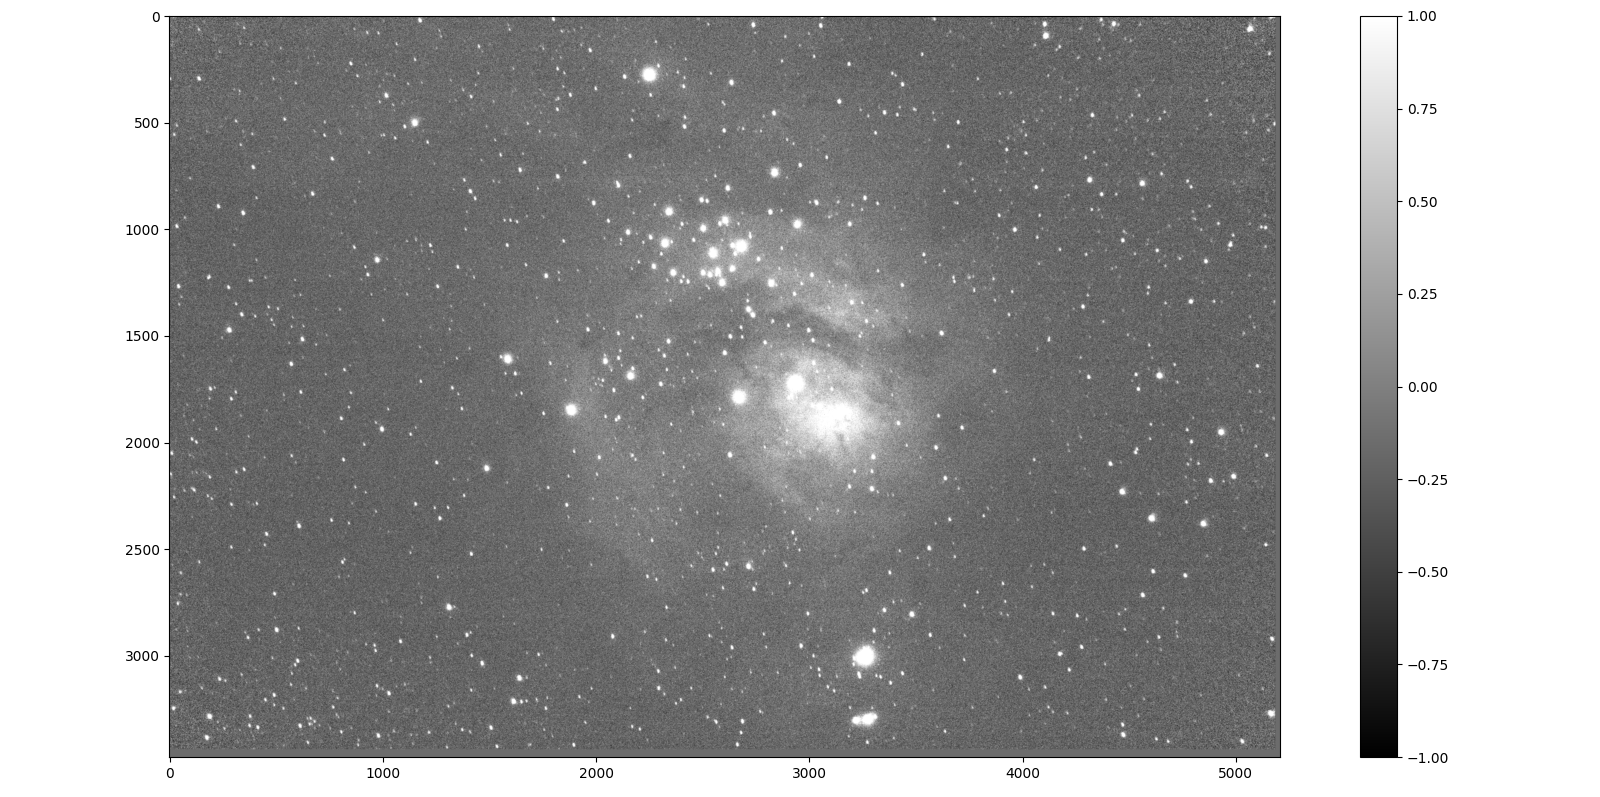
\includegraphics[width=\textwidth]{img/sin_proc.png}
  \caption{\label{fig:laguna0} Toma científica de la Nebulosa Laguna (M8) sin procesar, con el histograma reescalado entre los percentiles 2 y 98. Los números en los ejes indican coordenadas en pixeles. La barra lateral indica los niveles de brillo del histograma.}
\end{figure}

Luego de ejecutar el programa completo, con apilado por promedio simple de pixeles en las tomas ya calibradas y alineadas, se obtuvo la imagen que se muestra en la Figura~\ref{fig:apiladofinal}. Obsérvese nuévamente en la región  de pixeles de coordenadas $(1500, 2000)$: alrededor de la estrella que se observaba antes ``aislada'', ha aparecido una región oscura que antes apenas se apreciaba. La nebulosa se halla mucho más definida. Algo importante a observar es que no hay indiciones de que el registrado sea deficiente. Esto se evidencia en que las estrellas de la imagen final no se han deformado, comparativamente con las tomas originales.

\begin{figure}[!h]
  \centering
  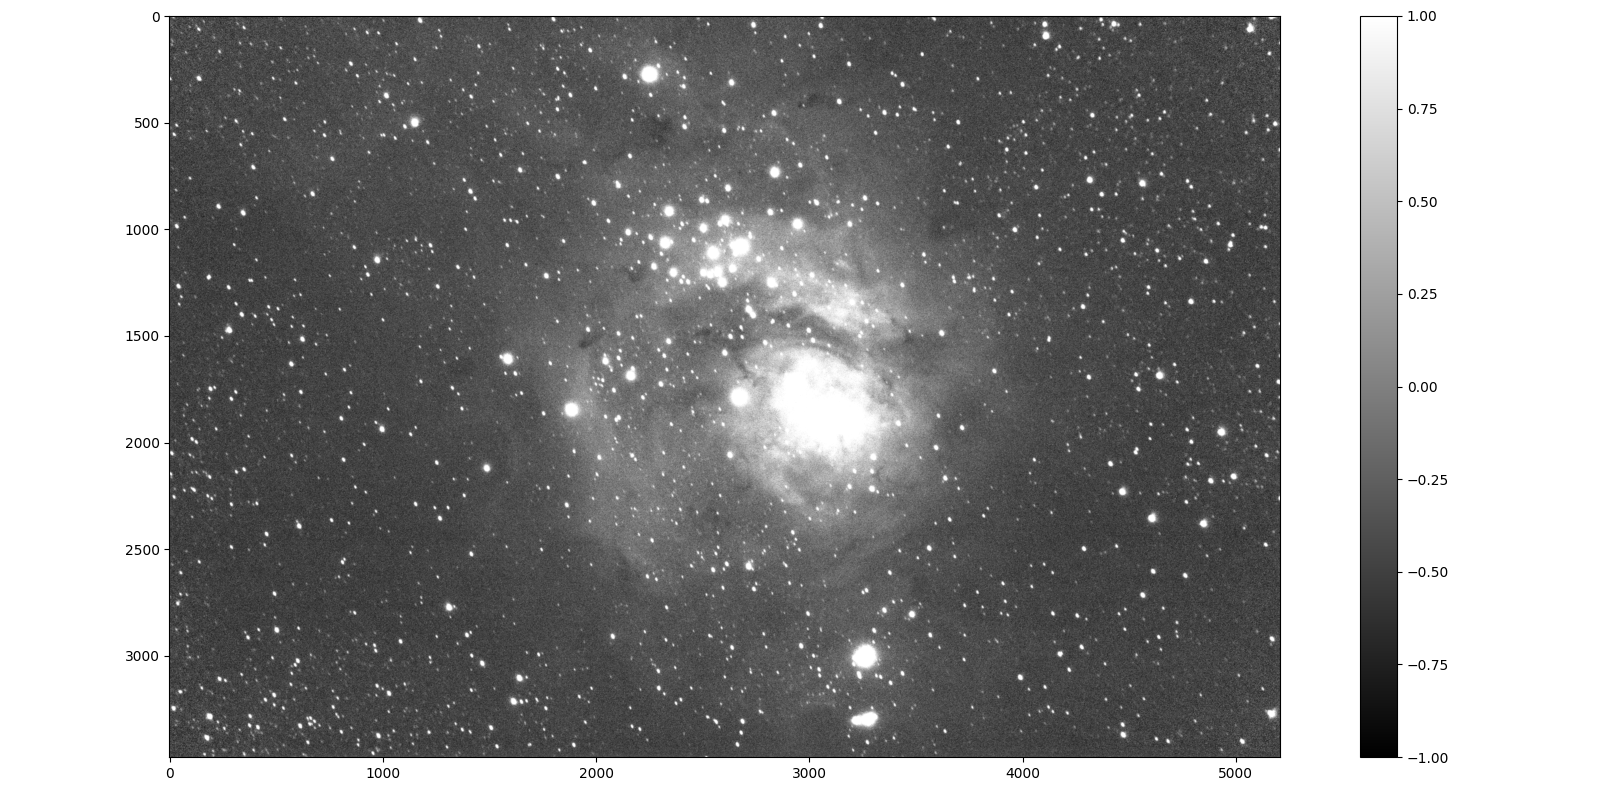
\includegraphics[width=\textwidth]{img/apiladofinal_scikit.png}
  \caption{\label{fig:apiladofinal} Imagen apilada de la Nebulosa Laguna (M8), con el histograma reescalado entre los percentiles 2 y 98. Los números en los ejes indican coordenadas en pixeles. La barra lateral indica los niveles de brillo del histograma. Esta imagen está compuesta por 9 tomas científicas, 20 tomas Bias, 10 Dark y 15 Flat.}
\end{figure}



\begin{figure}[!h]
  \centering
  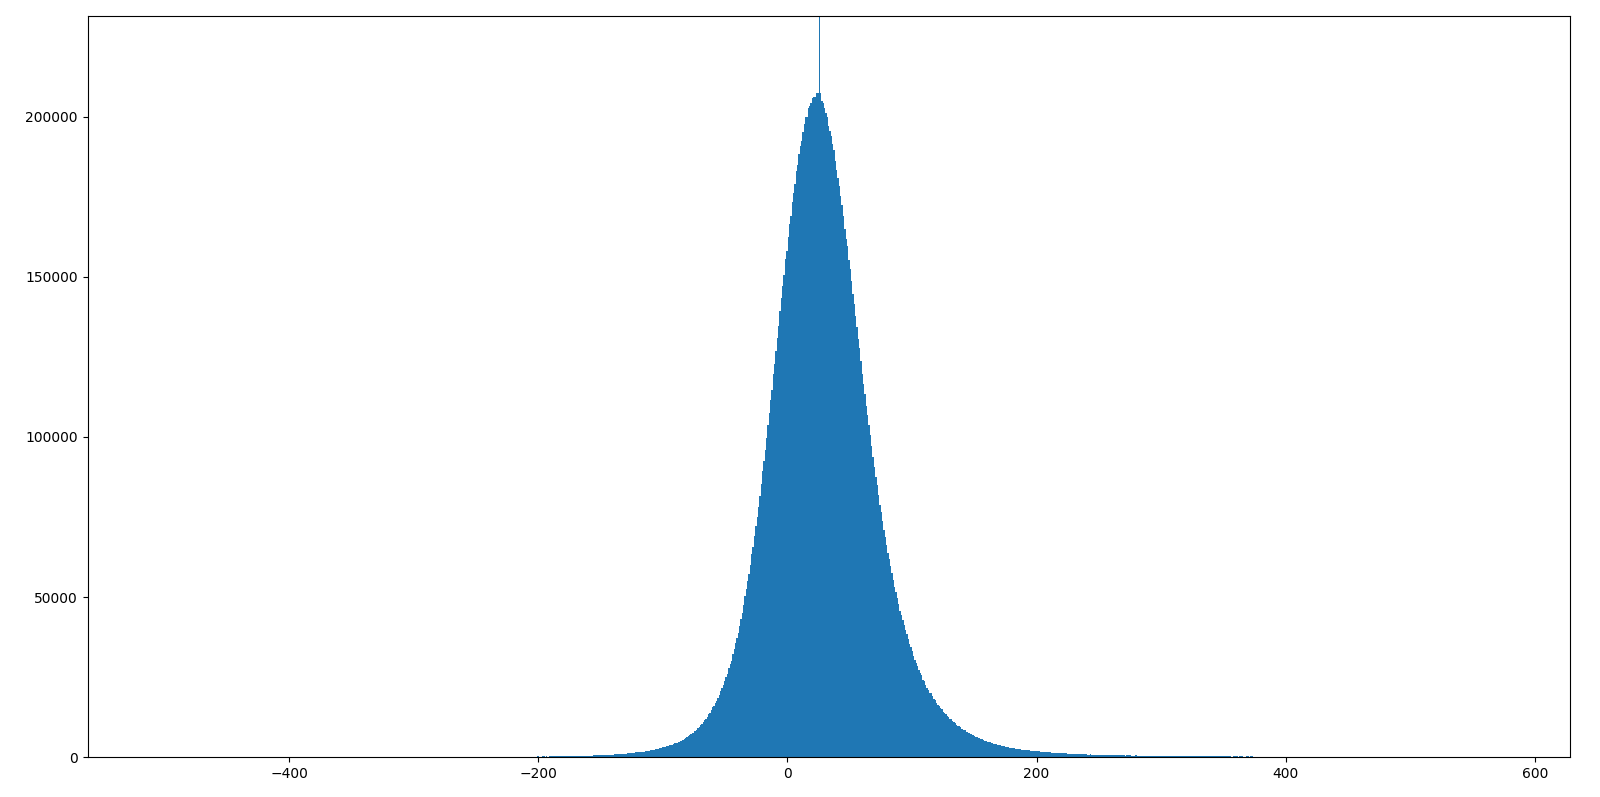
\includegraphics[width=\textwidth]{img/histo_00004.png}
  \caption{\label{fig:histo_sp} Histograma de la imagen sin procesar de la Figura~\ref{fig:laguna0}. La region de interés está ampliada para notar detalles de la distribución.}
\end{figure}

\begin{figure}[!h]
  \centering
  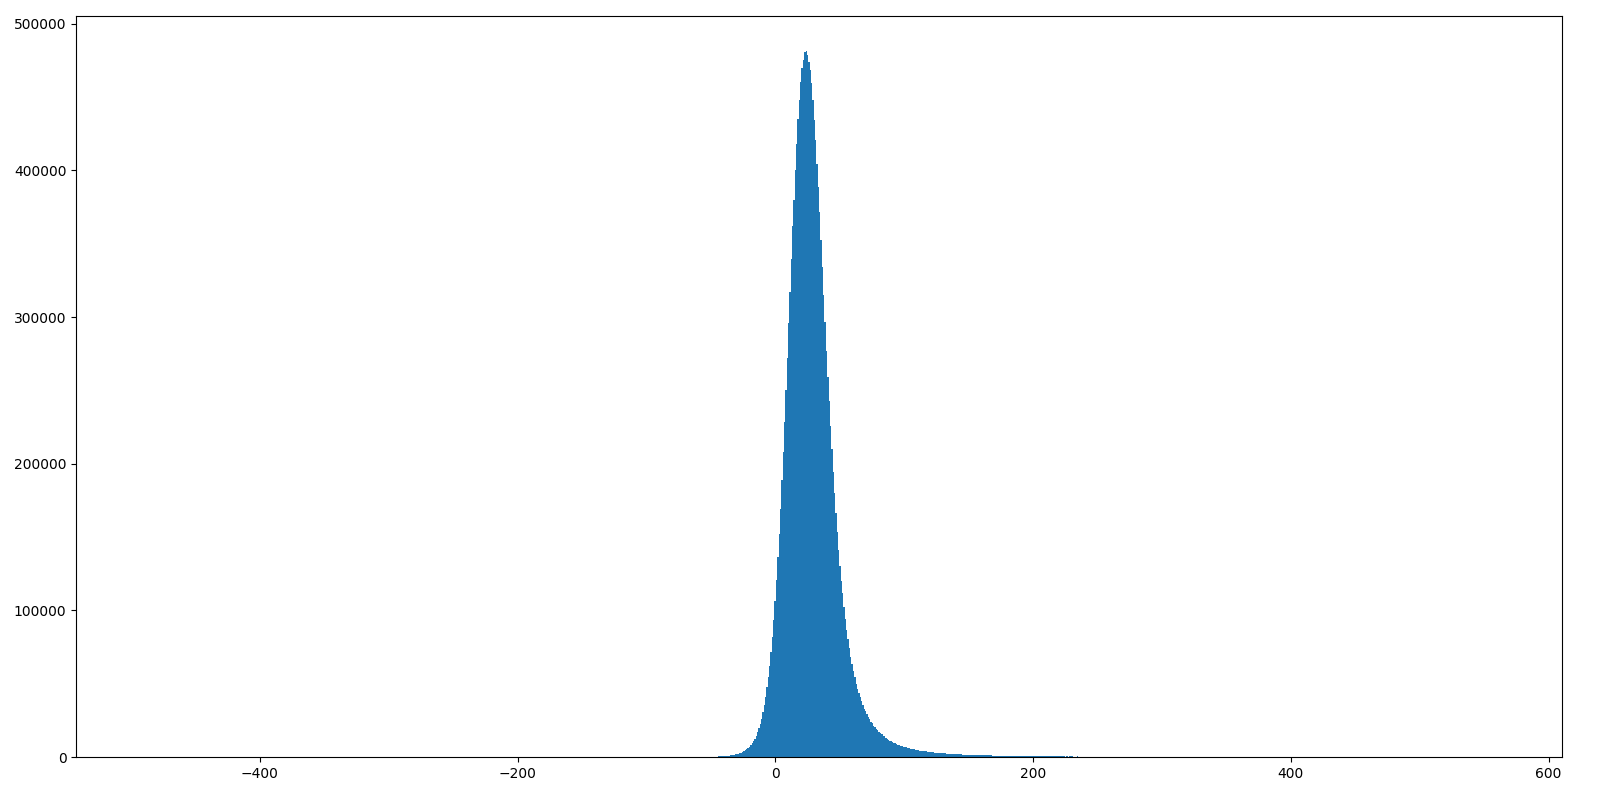
\includegraphics[width=\textwidth]{img/histo_final.png}
  \caption{\label{fig:histo_proc} Histograma de la imagen final procesada de la Figura~\ref{fig:apiladofinal}. La region de interés está ampliada para notar detalles de la distribución.}
\end{figure}

A los fines de comparar en forma más cuantitativa las dos imágenes, la Figura~\ref{fig:histo_sp} muestra el histograma de la imagen sin procesar, mientras que la Figura~\ref{fig:histo_proc} muestra el histograma de la imagen final apilada. Se observa que en el histograma de la imagen sin apilar, la distribución tiene una dispersión mayor que en el histograma de la imagen final. Esta mayor dispersión en la imagen sin procesar, visible en el ancho del pico y en su altura, es consistente con una presencia de mayor ruido en la imagen.

Una forma posible de probar la calidad de todo el proceso es medir la relación señal/ruido (SNR). Como se ha explicado en la sección \label{sec:tomas}, la reducción de imágenes debería incrementar la SNR, y también lo debería hacer el apilado. Para verificar que esto efectivamente se cumple con el procesado realizado con PyReduc, se ha realizado el siguiente procedimiento:

\begin{enumerate}
\item Se seleccionó un área cuadrada arbitraria de la imagen, de $50\times50=2500$ pixeles que mostrara el fondo del cielo (sin objetos astronómicos visibles). La esquina superior izquierda de dicha área estaba ubicada coordenadas $(400,400)$.
\item Se midió para el área elegida el valor promedio $\mu_{bg}$ y su desviación estándar $\sigma_{bg}$.
\item Se eligió una estrella arbitraria, no saturada, en la imagen\footnote{En un trabajo previo, fuera del alcance de este trabajo, se determinó que la cámara utilizada para estas pruebas perdía linealidad a las 15815 ADU. Estrellas en la imagen con valores ADU mayores que ese, estarán saturadas.}, y utilizando un cuadrado de  $50\times50=2500$ pixeles se midió el valor promedio $\mu_s$. La resta $\mu_s - \mu_{bg}$ representa la amplitud de de la señal, eliminando el ruido, mientras que la desviación estándar del fondo del cielo representa el ruido.
\item Se calculó la relación señal/ruido en decibeles como $$\mbox{SNR}=10 \log{\left(\frac{\mu_s - \mu_{bg}}{\sigma_{bg}}\right)}$$ Aunque hay diferentes definiciones para la SNR, en este trabajo se eligió esta definición, algo diferente de la de la bibliografía \cite{easton, romanishin}, por su practicidad a la hora de medir, sin necesidad de tomas de referencia o de calcular parámetros de la cámara.
\end{enumerate}

En la Figura~\ref{fig:snr} se muestra una gráfica de las mediciones de SNR realizadas con el proceso antes descripto, incrementando la cantidad de tomas científicas a apilar de a una por vez. También se incluyen las mediciones de una toma sin reducir, y de una sola toma reducida con Bias, Dark y Flats. Se observa que, efectivamente, una toma reducida tiene una mayor SNR que una toma sin reducir. Además se observa que a medida que se apilan más tomas, la SNR aumenta. Comprobamos así que el apilado, con el conjunto de imágenes de prueba aquí utilizado, mejora la SNR.  Aunque, debido a la pequeña cantidad de imágenes apiladas, este procedimiento no pretende ser preciso, se ha determinado una relación experimental entre la SNR y la cantidad de tomas científicas $x$: $$\mbox{SNR}=17.9(x-0.77)^{0.054}$$ Las incertezas de esta determinación se presentan junto con el ajuste no lineal en la Figura~\ref{fig:snr}. Queda pendiente comprobar que esta tendencia de mejora de la SNR al aumentar el número de tomas se sigue cumpliendo al apilar un mayor número de tomas científicas, digamos entre 50 y 100 tomas.


\begin{figure}[!h]
  \centering
  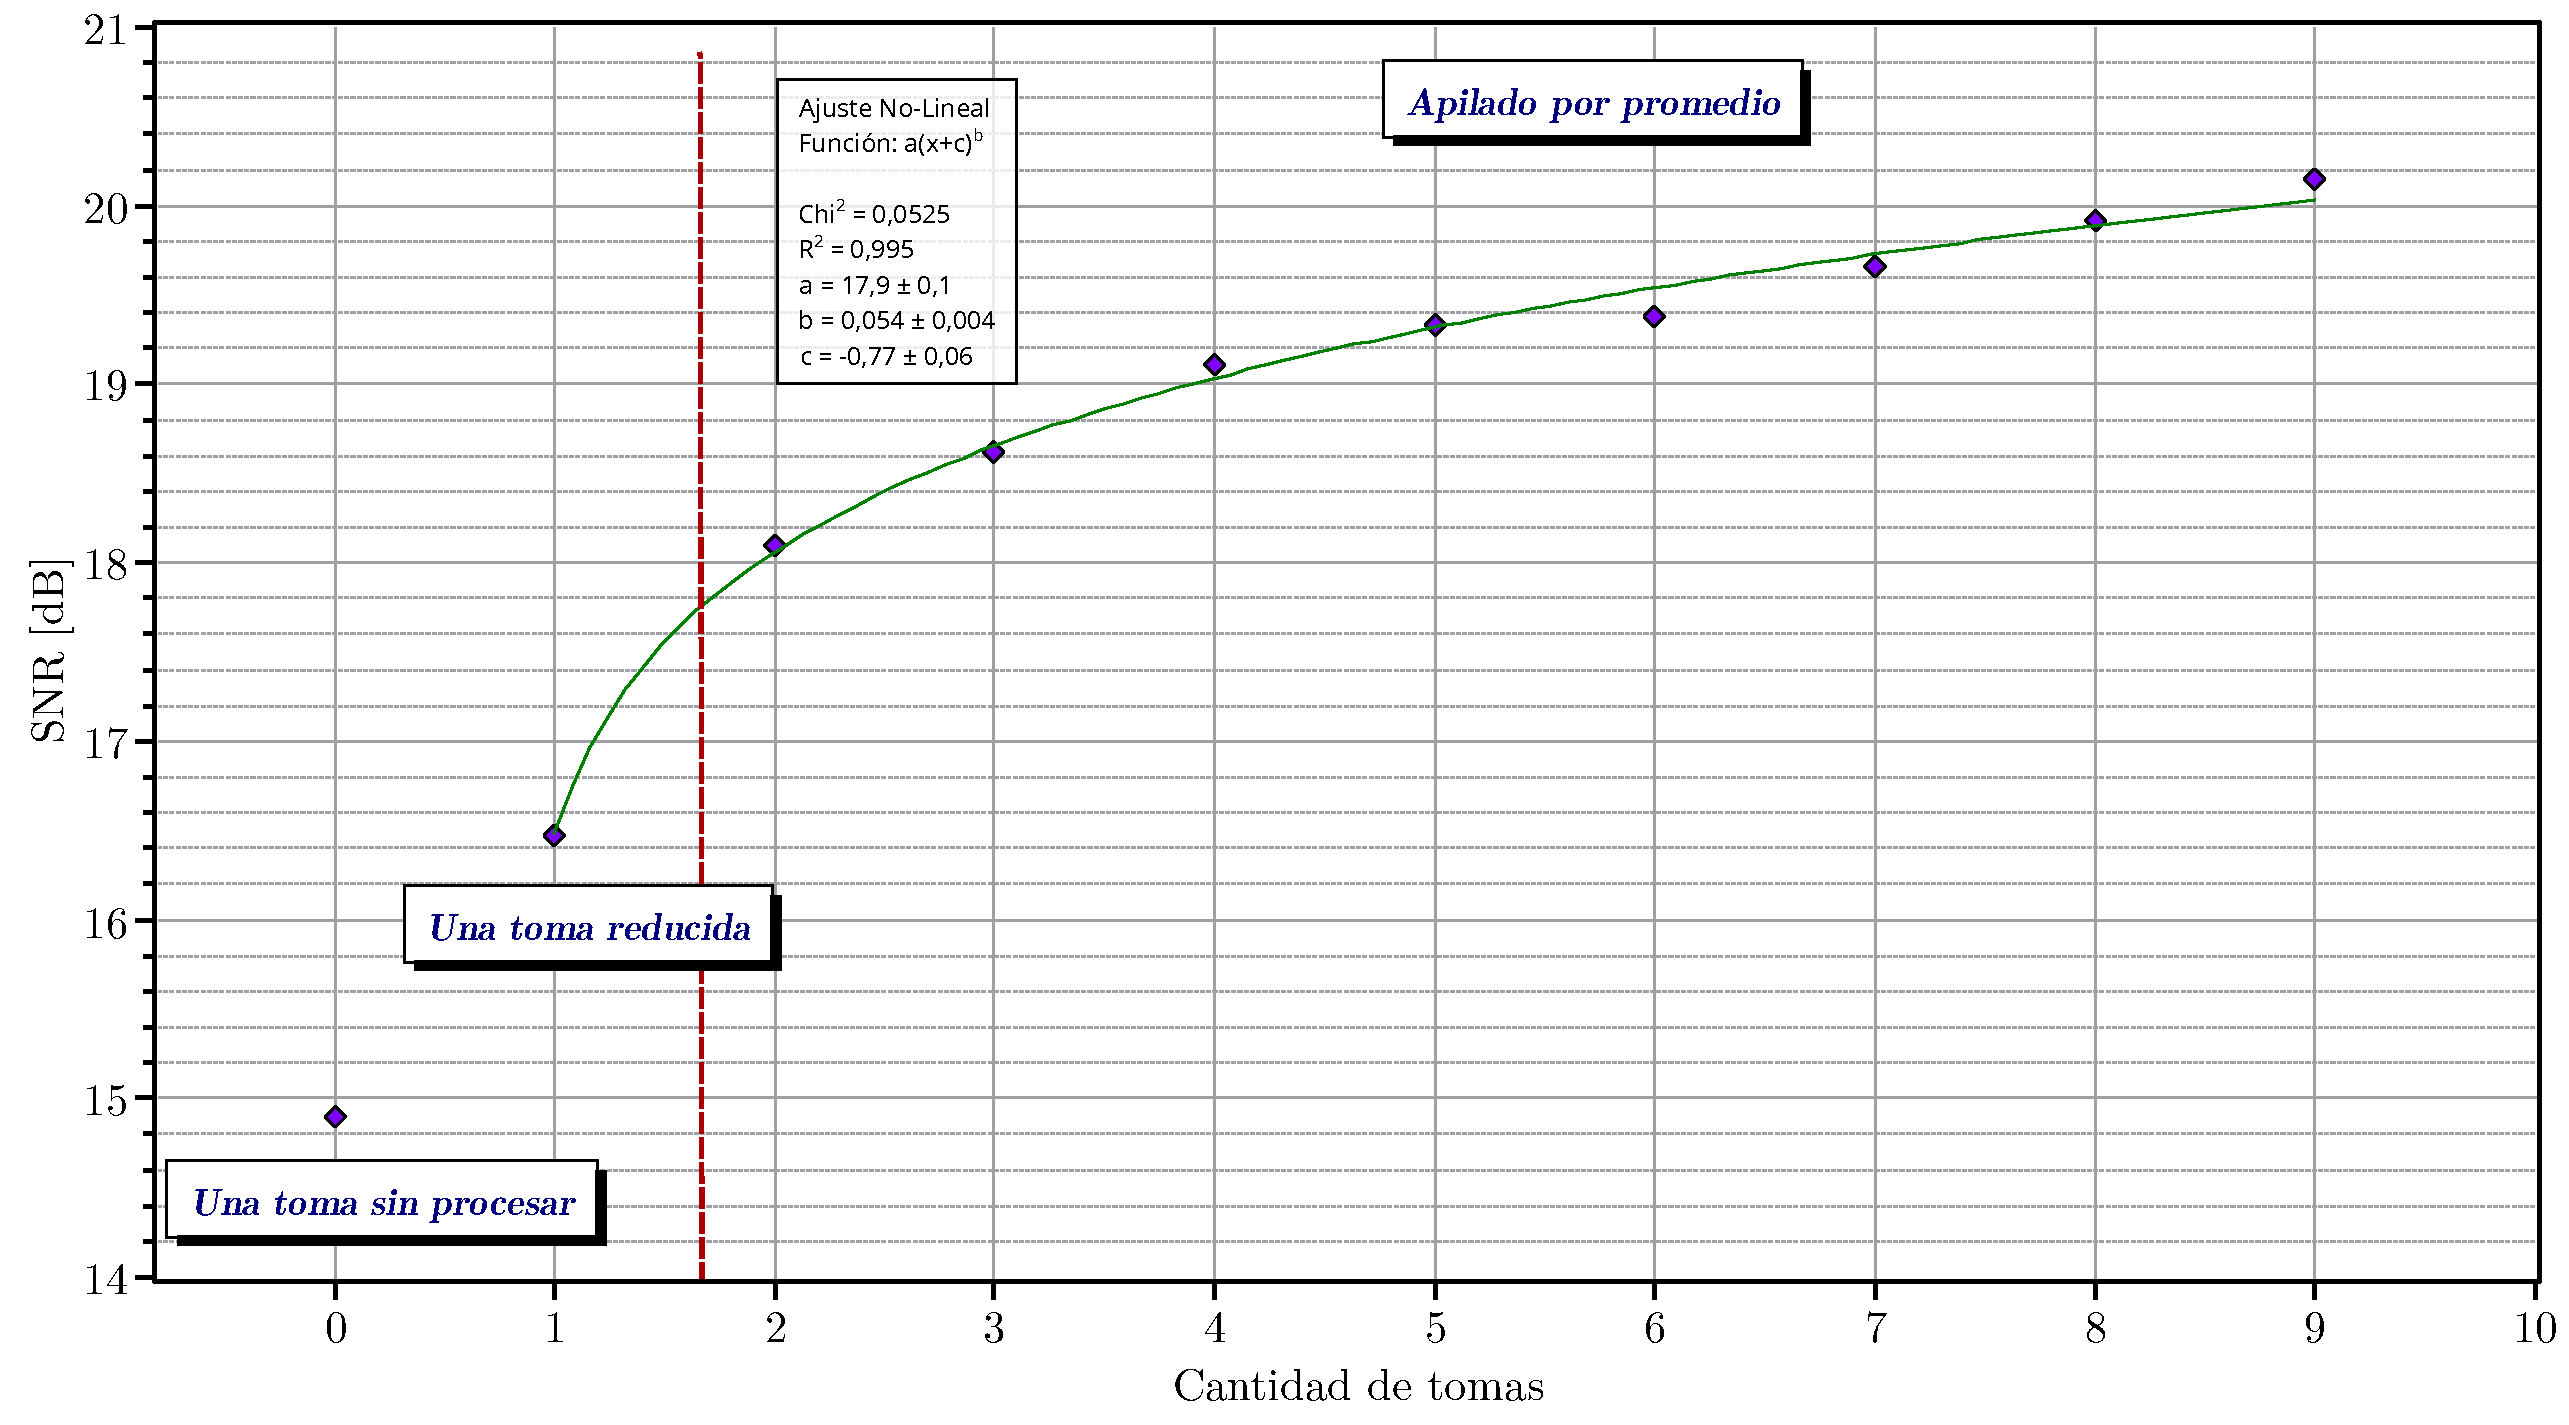
\includegraphics[width=\textwidth]{img/SNR.pdf}
  \caption{\label{fig:snr} Relación señal/ruido (SNR) en función de la cantidad de tomas científicas apiladas. Se nota una mejora de la SNR a medida que se van agregando más tomas científicas. El valor de cero en las absisas indica una sola toma sin reducir, mientras que el valor uno indica una sola toma reducida por Bias, Dark y Flats.}
\end{figure}


Luego de estas primeras pruebas, se verificó el funcionamiento del algoritmo de apilado con descarte de valores extremos (Pixel Rejection). Aunque el algoritmo funcionó correctamente, se encontró que el tiempo de ejecución era súmamente largo, en comparación con el del promedio simple, o con el realizado por otros softwares. En una computadora {\sf intel CORE i7 7th Gen} con 16 GB de RAM, el tiempo de ejecución de este algoritmo fue de 55 min. En este caso, para obtener resultados más rápidos, sería necesario paralelizar este proceso, para que el trabajo de recorrer el arreglo de imágenes a apilar no sea tan lento. Por otro lado, en la instancia de visualización, no se encontraron diferencias significativas entre las imágenes resultantes de los dos métodos de apilado.

Finalmente, se realizó una comparativa de los tres métodos de visualización. En la Figura~\ref{fig:visual} se muestran los tres métodos juntos. 

\begin{figure}[!h]
  \centering
  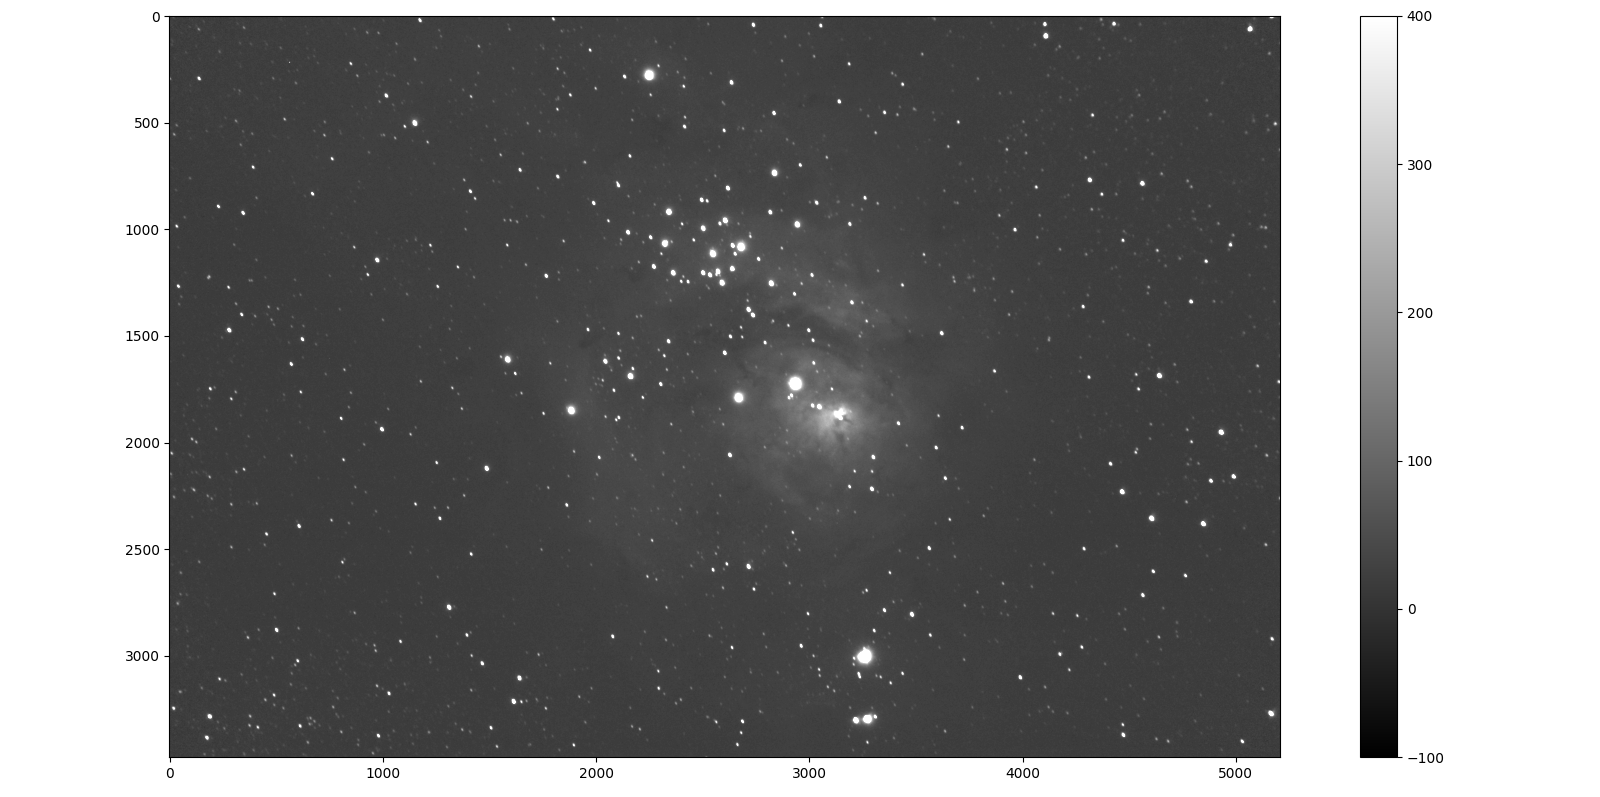
\includegraphics[width=0.8\textwidth]{img/Figure_Manual.png}
  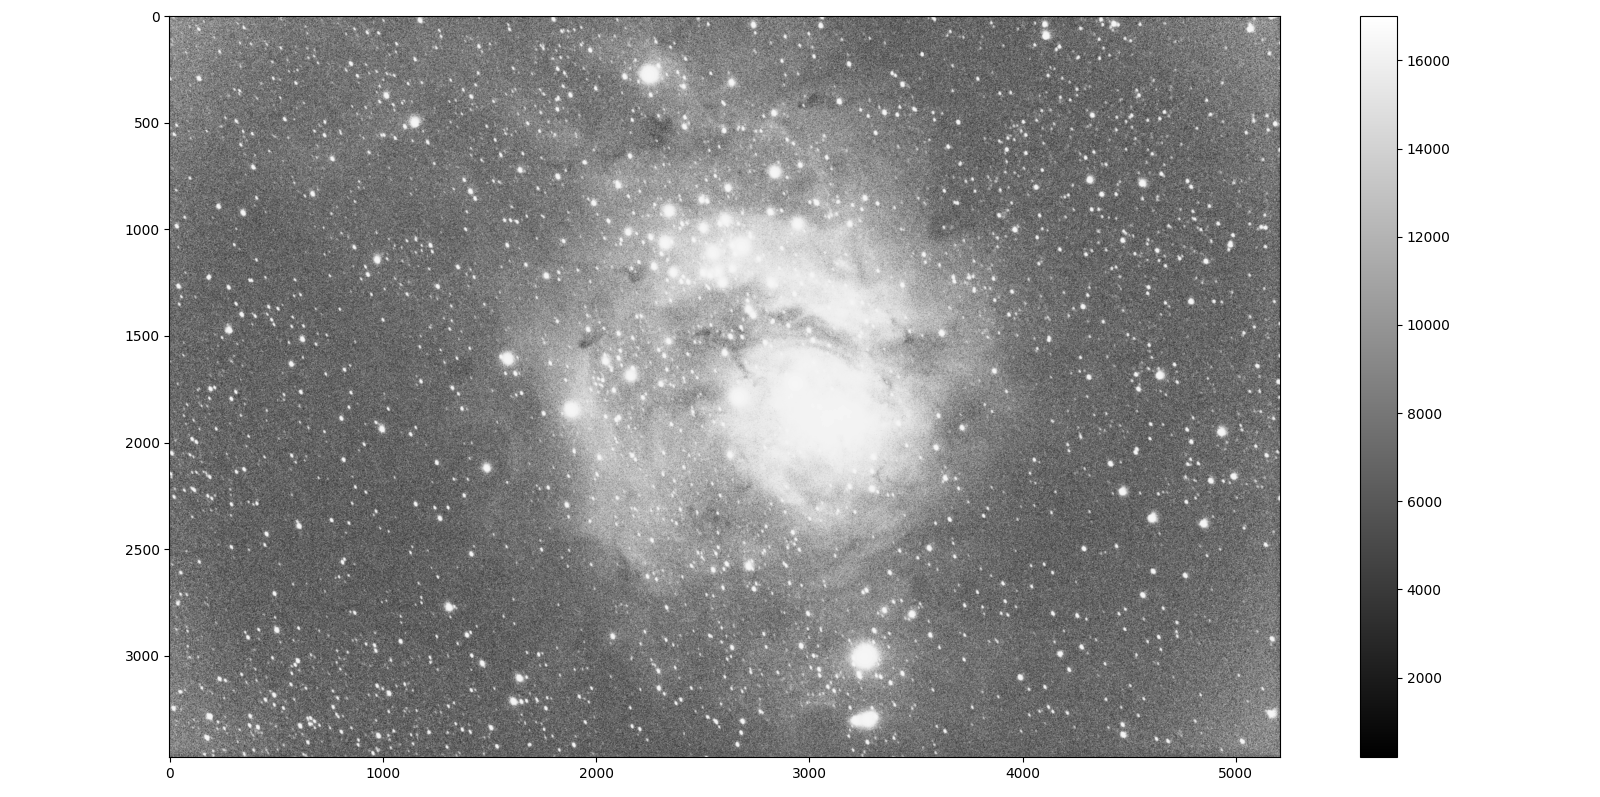
\includegraphics[width=0.8\textwidth]{img/Figure_Ecualizado.png}
  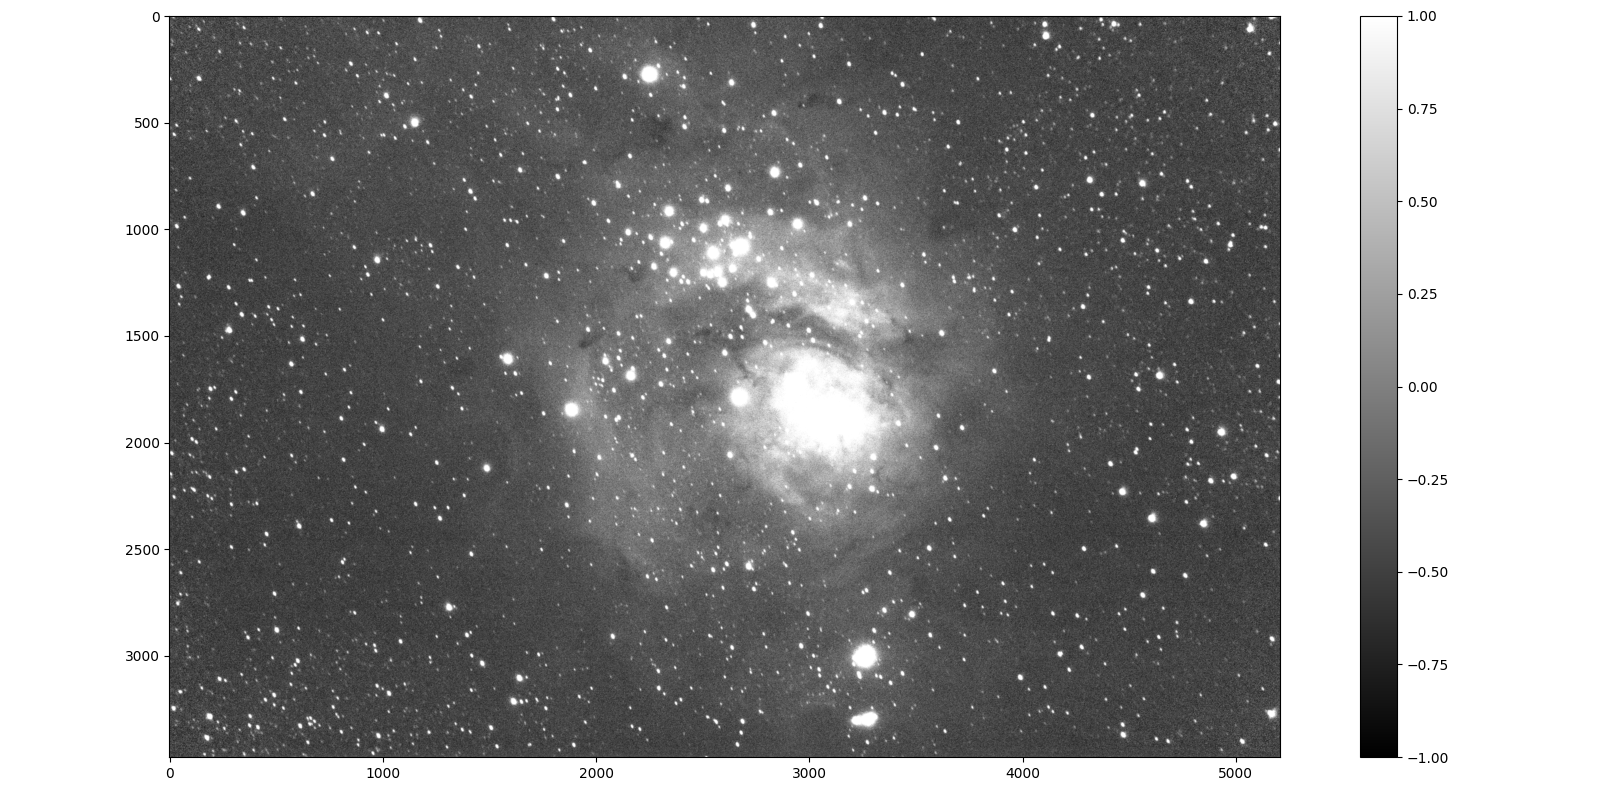
\includegraphics[width=0.8\textwidth]{img/apiladofinal_scikit.png}
  \caption{\label{fig:visual} Comparación de los tres modos de visualización que ofrece PyReduc. En el centro, recorte manual entre los valores -100 y 400 del histograma. En el medio, ecualización automática de PyReduc. Abajo,  reescalado entre los percentiles 2 y 98, utilizando la librería scikit.}
\end{figure}

Es importante notar la diferencia entre las escalas de niveles de gris que se presentan a la derecha de cada imagen para comprender lo que hace cada modo de visualización. En el caso del recorte manual (Figura~\ref{fig:visual}, arriba), al usuario se le presenta un histograma, en este caso, el de la Figura~\ref{fig:histo_proc}, y este elige entre qué valores recortar. Para esta prueba, se ha elegido el intervalo $[-100,400]$ para mostrar la imagen, y eso es lo que puede verse en la barra lateral. En este caso, entonces, el valor $-100$ corresponde al negro y el valor $400$ al blanco. La imagen resultante no revela muchos detalles de la nebulosa, por lo que el usuario poco experimentado se verá obligado a intentar diferentes juegos de valores extremos para mejorar la imagen que obtiene por pantalla.

En el caso de la ecualización automática (Figura~\ref{fig:visual}, en el centro), como se explica en el Apéndice \ref{sec:ecualizado}, el algoritmo {\it mapea} el histograma a uno nuevo, más aplanado. El rango de niveles de gris en este algoritmo es el mismo que en la imagen original, y eso se observa en la escala, a la derecha de la imagen. En este proceso de ecualización, se maximiza la información que muestra la imagen, notándose muchos detalles que no aparecen en las otras formas de visualización. Algunos detalles son inesperados, como por ejemplo, la presencia de algo que podríamos llamar {\it ``viñeteo inverso''}: las esquinas de la imagen se ven más claras como resultado de corregir la imagen con flats en exceso. Dado que este exceso no aparece en las otras formas de visualización, se juzga como aceptable la calibración realizada. El algoritmo de ecualizado implementado resultó ser muy rápido. Una desventaja esperable de este método de visualización es que la imagen aparece, como se dice en la jerga de la fotografía astronómica, {\it muy lavada}, con lo cual se pierde la noción de la relación de magnitudes entre las estrellas de la imagen.

Finalmente, en el caso del reescalado automático entre los percentiles 2 y 98, vemos que esta función recorta la información entre dichos percentiles y luego mapea los datos a una nueva escala de grises entre los valores $-1$ y 1.
Aunque en esta visualización, el núcleo de la nebulosa queda muy saturado, a los fines de visualizar detalles de la imagen es un procedimiento muy efectivo.

Vale la pena insistir aquí en que estos métodos de visualización, cada uno con sus bondades y sus limitaciones, son solo una forma de que el usuario evalúe el resultado final de todo el proceso, y no tienen utilidad fotométrica. Es por ello que ninguno de los tres se guarda automáticamente en archivo. Los cambios en el histograma se realizan en la memoria RAM y, al cerrar la ventana de visualización, se pierden.

Para cerrar esta sección, se ha probado de abrir las imágenes obtenidas con PyReduc en otro software. Por ejemplo, se han abierto satisfactoriamente con ImageJ y con su versión astronómica AstroImageJ. Estos softwares se usan de forma profesional en varias Universidades y Observatorios del mundo \cite{craig}. Por otro lado, debido a la conversión que realiza la librería \texttt{astropy.io.fits} de imágenes al formato de 32 bits con signo, no ha sido posible abrir satisfactoriamente las imágenes de PyReduc con softwares de tipo amateur como Iris o Siril.

\section{Conclusiones y perspectivas}
En este trabajo se comentaron las funciones que se implementaron en el software PyReduc para reducción y apilado de imágenes astronómicas DSLR. Se probaron estas funciones con una serie de tomas científicas y de calibración de la nebulosa Messier 8 en el canal verde, con las cuales se comprobó que el software es adecuado para el proceso de reducción de imágenes DSLR monocromáticas. El alineado resultó satisfactorio en las imágenes utilizadas. El apilado de imágenes por promedio simple resultó ser eficiente. Se comprobó que a través de este procedimiento se obtiene un incremento en la relación señal/ruido, cumpliéndose así el objetivo del apilado.
En cuanto a la visualización final, los tres métodos implementados funcionaron adecuadamente. Aunque cada uno presenta diferentes limitaciones, estas se hallan dentro de lo esperado y estas no son un problema pues su utilidad radica en una visualización rápida de las imágenes obtenidas.

Como perspectivas a futuro, se espera incorporar un algoritmo que permita importar las imágenes RAW a FITS y extraer un canal sin depender de un software externo para este fin. Es importante seguir testeando PyReduc con más imágenes, para testear todas las funciones del software. Además se espera poder reemplazar el algoritmo de apilado con descarte de pixeles extremos (Pixel Rejection) por uno que se ejecute más eficientemente, a los fines de obtener aun más mejoras en la relación señal/ruido. Finalmente, dado que el objetivo de PyReduc es la reducción de imágenes con fines fotométricos, el próximo paso a llevar a cabo es probar las imágenes reducidas y apiladas con algún software de fotometría. Se ha verificado que las imágenes de PyReduc se pueden abrir con AstroImageJ, software que se está usando profesionalmente para este fin, pero aún no se ha dado el paso de realizar mediciones fotométricas.

   

\begin{thebibliography}{100}
\bibitem{aavso} American Association of Variable Star Observers: {\it ``Manual de Observación DSLR de AAVSO''}, Versión 1.1 en Español, 2015. En Internet: \url{https://www.aavso.org/dslr-observing-manual}
  \bibitem{fsf} Free Software Foundation: {\it ``Qué es el software libre?''}, Versión 1.153, 2017. En Internet: \url{https://www.gnu.org/philosophy/free-sw.es.html}
\bibitem{greisen} Eric W. Greisen: {\it ``FITS: a remarkable achievement in information exchange''}, 2003. En: Heck A. (eds) Information Handling in Astronomy - Historical Vistas. Astrophysics and Space Science Library, vol 285. Springer, Dordrecht. \url{https://doi.org/10.1007/0-306-48080-8_5}
\bibitem{phillips} Dwayne Phillips: {\it ``Image Processing in C''}, 2nd Ed, 2000. En Internet: \url{http://homepages.inf.ed.ac.uk/rbf/BOOKS/PHILLIPS/cips2ed.pdf}
\bibitem{gil-hutton} Ricardo Gil-Hutton: {\it ``Cómo hacer una reducción básica de imágenes FITS con Python''}, Noviembre 2016. En Internet: \url{https://freeshell.de/~rgh/arch/python/python-red-basica.pdf}
\bibitem{nasa} The FITS Support Office: {\it ``What is FITS?''}, NASA. Última revisión, Diciembre 2017.  En Internet: \url{https://fits.gsfc.nasa.gov/}
\bibitem{fits} FITS Working Group, International Astronomical Union: {\it ``Definition of the Flexible Image Transport System (FITS)''}, Version 4.0, 2016. En Internet: \url{https://fits.gsfc.nasa.gov/standard40/fits_standard40aa-le.pdf}
\bibitem{craig} Matthew Craig, Juan Cabanela, Linda Winkler: {\it ``Introduction to Astronomical Image Analysis''}, 2014. En Internet: \url{https://image-analysis.readthedocs.io}
\bibitem{brown} Lisa G. Brown: {\it ``Image Registration Techniques''}, ACM Computmg Surveys, Vol 24, No. 4, 1992. \url{https://doi.org/10.1145/146370.146374}
\bibitem{astropy} Astropy Collaboration: {\it ``The Astropy Project: Building an Open-science Project and Status of the v2.0 Core Package''}, The Astronomical Journal, Volume 156, Issue 3, article id. 123, 19 pp., 2018. \url{https://doi.org/10.3847/1538-3881/aabc4f}
\bibitem{aydin}  M. Emre Aydin: {\it ``cr2fits v2''}, Version v2.1.0, 2017, May 21, Zenodo. \url{http://doi.org/10.5281/zenodo.581722}
\bibitem{astroalign} Martin Beroiz: {\it ``toros-astro/astroalign''}, Version v1.0.3, 2018, May 18. Zenodo. \url{http://doi.org/10.5281/zenodo.1249048}
\bibitem{easton} Roger L. Easton Jr.: {\it ``Fundamentals of Digital Image Processing''}, Noviembre de 2010, Chester F. Carlson Center for Imaging Science, Rochester Institute of Technology. \url{https://www.cis.rit.edu/class/simg361/Notes_11222010.pdf}
\bibitem{romanishin} W. Romanishin: {\it ``An Introduction to Astronomical Photometry Using CCDs''},  Octubre de 2006, University of Oklahoma, En Internet: \url{http://www.physics.csbsju.edu/370/photometry/manuals/OU.edu_CCD_photometry_wrccd06.pdf}
\end{thebibliography}




\newpage
\appendix

\section{Apéndice}
\subsection{Listado del código principal de PyReduc}
En esta sección se lista el código contenido en el archivo {\tt pyreduc.py}, módulo principal de PyReduc.
\begin{lstlisting}[style=python]
#!/usr/bin/python3

"""
PyReduc
Programa de reducción de imágenes FITS
Autor: Carlos Mauricio Silva
Versión: 0.2.5

Licencia GNU GENERAL PUBLIC LICENSE
Leer archivo LICENSE que se distribuye con este programa.

Parte del código de calibración con Darks/Bias/Flats está basado en el Tutorial "Cómo hacer una reducción básica de imágenes FITS con Python" de Ricardo Gil-Hutton. Este tutorial estaba basado en la librería PyFits, que ya no se usa y ha sido reemplazada por astropy.io.fits.
La fórmula de reducción de imágenes científicas que se utiliza aquí fue tomada del curso "Introduction to Astronomical Image Analysis" de  Matthew Craig, Juan Cabanela & Linda Winkler.
"""

import numpy as np
from astropy.io import fits as ft
import glob
import os, shutil
from pathlib import Path

import apilado
import registrado
import visualizacion

# Presentación
print("_______________________________________")
print("PyReduc")
print("\nPrograma de reducción de imágenes FITS")
print("Autor: Carlos Mauricio Silva")
print("Versión: 0.2.0")
print("_______________________________________")
print("\nLas imágenes FITS deben estar en un directorio llamado")
print('''"pyreduc/FITS/", dentro del directorio home.''')
print("Los prefijos de los archivos deben seguir las siguientes reglas:")
print(''' FLATS: "flat*"\n DARKS: "dark*"\n BIAS: "bias*" \ndonde "*" significa "cualquier cosa". El prefijo de los LIGHTS se ingresa por teclado\n''')

# Averiguo el nombre del directorio home
home = str(Path.home())

#################
### FUNCIONES ###
#################


def copia_de_imagenes():
    # Hago una copia de todos los archivos para no sobreescribir los FITS
    # En la carpeta ~/pyreduc/procesado/
    home = str(Path.home())
    os.chdir(home+"/pyreduc/FITS")
    origen = os.getcwd()
    destino = home+"/pyreduc/procesado/"
    ignorar_pat = shutil.ignore_patterns('*.seq')
    if os.path.exists(destino): # Si el directorio destino existe, lo elimino con todo su contenido
        print("Antes de empezar a trabajar, se borrará el directorio ~/pyreduc/procesado/")
        input("Para cancelar la operación presione Ctrl+C. Para continuar presione Enter")
        shutil.rmtree(destino)
        print("Aguarde mientras se crea una copia de sus imágenes\n") 
        try:                   # Y ahora lo vuelvo a crear copiando todas las imagenes allí     
            arbol = shutil.copytree(origen, destino, ignore=ignorar_pat) 
            print('Todas las imágenes se han copiado a', arbol)
        except:
            print('Error en la copia')
    else:
        print("Aguarde mientras se crea una copia de sus imágenes\n") 
        try:                        
            arbol = shutil.copytree(origen, destino, ignore=ignorar_pat) 
            print('Todas las imágenes se han copiado a', arbol)
        except:
            print('Error en la copia')


def mediana_calib(listaimg,numimg):
    # Genero una matriz 3D de ceros
    cubo_nuevo=np.zeros((numimg,ft.getval(listaimg[0],'naxis2'),ft.getval(listaimg[0],'naxis1')),dtype=float)
    # Copio las tomas de calibración a la matriz cúbica
    nro=0
    for ii in listaimg:
        ff=ft.open(ii)
        img=ff[0].data
        hdr=ff[0].header
        ff.close()
        cubo_nuevo[nro,:,:]=np.copy(img)
        nro+=1
        
    # Ordeno los pixeles de menor a mayor a lo largo del primer eje.
    cubo_nuevo=np.sort(cubo_nuevo,axis=0)
    
    # Creo una nueva imagen con el valor de la mediana, despreciando el valor más alto de cada pixel.
    return np.median(cubo_nuevo[0:numbias-1],axis=0)


            
def resta_master(lista,stacked_img):
    for ii in lista:
        ff=ft.open(ii)
        img=ff[0].data
        hdr=ff[0].header
        ff.close()
        img=img-stacked_img
        hdr.add_comment("Procesado por DARK y BIAS con PyReduc")
        ft.writeto(ii,img,header=hdr,overwrite=True)  # overwrite=True va a sobreescribir cada archivo.


#####################
### FIN FUNCIONES ###
#####################

copia_de_imagenes() # Llamo a la función que me backupeará las imágenes

# Voy al directorio donde están las imágenes copiadas
os.chdir(home+"/pyreduc/procesado")

# Pido al usuario el prefijo de los archivos light
print("\nComenzando a trabajar con sus imágenes en el directorio", os.getcwd())
prefijo=input("\nIntroduzca el prefijo de los archivos lights (tomas científicas): ")

# Construyo listas de tomas dark, bias, flat y lights
lista_dark=glob.glob("dark*.fit")
lista_bias=glob.glob("bias*.fit")
lista_flat=glob.glob("flat*.fit")
lista_lights=glob.glob(prefijo+"*.fit")

print("\n")
print("Archivos DARK:\n")
for ii in lista_dark:
    print("{:}: {:}x{:}  EXPTIME={:} s".format(ii,ft.getval(ii,'naxis2'),ft.getval(ii,'naxis1'),ft.getval(ii,'exptime')))

print("\n")
print("Archivos BIAS:\n")
for ii in lista_bias:
    print("{:}: {:}x{:}  EXPTIME={:} s".format(ii,ft.getval(ii,'naxis2'),ft.getval(ii,'naxis1'),ft.getval(ii,'exptime')))    

print("\n")
print("Archivos FLAT:\n")
for ii in lista_flat:
    print("{:}: {:}x{:}  EXPTIME={:} s".format(ii,ft.getval(ii,'naxis2'),ft.getval(ii,'naxis1'),ft.getval(ii,'exptime')))    

print("\n")
print("Archivos LIGHTS (tomas científicas):\n")
for ii in lista_lights:
    print("{:}: {:}x{:}  EXPTIME={:} s".format(ii,ft.getval(ii,'naxis2'),ft.getval(ii,'naxis1'),ft.getval(ii,'exptime')))

print("\nTenga en cuenta que para la calibración se toma el tiempo de exposición de su primer toma científica.")
print("PyReduc no dará los mejores resultados si sus tomas científicas tienen diferentes tiempos de exposición.")

continuar=input("Presione una tecla para continuar")

print("\nAl final del proceso se realizará un apilado de sus imágenes calibradas y alineadas. Este se puede realizar a través de un promedio simple de las imágenes, o con un promedio que rechace valores extremos (Pixel Rejection). ¿Qué desea hacer?")
print("1. Apilar promediando las imágenes")
print("2. Aplicar Pixel Rejection (POCO EFICIENTE. NO RECOMENDADO.)")
print("3. No apilar")
rechazar_pixel = input("Ingrese 1, 2 o 3: ")
while(rechazar_pixel not in ["1", "2", "3"]):
    print("Opción inválida")
    rechazar_pixel = input("Ingrese 1, 2 o 3: ")
    

# Guardo la cantidad de archivos de cada lista en una variable distinta:
numflat=len(lista_flat)
numbias=len(lista_bias)
numdark=len(lista_dark)
numlights=len(lista_lights)

# Voy a obtener el tiempo de exposición de los lights, flats y darks
# Voy a suponer que todas las tomas de un mismo tipo tienen la misma exposición.
exp_lights=ft.getval(lista_lights[0],'exptime')
exp_flat=ft.getval(lista_flat[0],'exptime')
exp_dark=ft.getval(lista_dark[0], 'exptime')

# Proceso de BIAS. Voy a armar una matriz cúbica de los bias.
print("\nProcesando BIAS. Por favor, aguarde...")

stbias = mediana_calib(lista_bias, numbias)


# Proceso de DARK.
print("\nProcesando DARK. Por favor, aguarde...")

# Primero, voy a restar un master-bias a los dark, para formar una lista de pre-DARK-current.
print("\nSustrayendo un master-bias a los dark. Aguarde...")
resta_master(lista_dark, stbias)

# Ahora realizo el apilado para generar la imagen Dark-current
stdark = mediana_calib(lista_dark, numdark)


# Ahora voy a crear una imagen que es la suma de DARK-current escalado y BIAS
# para corregir los lights
master_stack = stbias + stdark/exp_dark*exp_lights

# Resto la nueva imagen a los lights
resta_master(lista_lights, master_stack)


# para corregir los flats
master_stack = stbias + stdark/exp_dark*exp_flat

# Resto la nueva imagen a los flats
resta_master(lista_flat, master_stack)


# Proceso de FLATS. Voy a armar una matriz cúbica de los flats.
# Nótese que los flats ya fueron corregidos con bias y dark-current.
print("\nProcesando FLATS. Por favor, aguarde...")
# Genero una matriz 3D de ceros
cubo_flat=np.zeros((numflat,ft.getval(lista_bias[0],'naxis2'),ft.getval(lista_bias[0],'naxis1')),dtype=float)

# Copio los FLATS a la matriz cúbica
nro=0
sum=0
for ii in lista_flat:
    ff=ft.open(ii)
    img=ff[0].data
    hdr=ff[0].header
    ff.close()
    med=np.median(img)
    sum+=med
    cubo_flat[nro,:,:]=np.copy(img)*med
    nro+=1

# Creo una nueva imagen a partir de los valores medios, despreciando los valores más altos,
# pero normalizo con la suma de las medianas de cada imagen.
stflat=np.mean(cubo_flat[0:numflat-1],axis=0)/sum
mflat=np.mean(stflat)


# Divido las imágenes lights por el master-flat resultante.
for ii in lista_lights:
    ff=ft.open(ii)
    img=ff[0].data
    hdr=ff[0].header
    ff.close()
    img=img/stflat*mflat
    hdr.add_comment("Procesado por FLATS con PyReduc")
    ft.writeto(ii,img,header=hdr,overwrite=True)

   
# Alineación de imágenes:

registrado.registra_lista(lista_lights)

salir="1"

# Stacking o apilado de imágenes:
lista_lights=glob.glob(prefijo+"*.fit") # Reconstruyo la lista de lights
# Si el usuario pidio apilar, se apila, y si no, se sale del programa.
if(rechazar_pixel=="1" or rechazar_pixel=="2"):
    apilado.stacking(lista_lights, rechazar_pixel)
else:
    salir="2"


while(salir=="1"):
    print("¿Qué desea hacer?")
    print("1: Ver la imagen resultante")
    print("2: Salir")
    salir=input("Ingrese 1 o 2: ")
    if(salir=="1"):
        # Visualización por pantalla de la imagen:
        visualizacion.visual("stacking.fit")
    elif(salir=="2"):
        break
    else:
        print("Opción no válida")
        salir="1"

    
print("Gracias por utilizar PyReduc")

import gc
# Saco la basura y se la lleva el camión recolector
gc.collect()
\end{lstlisting}

\subsection{Listado del código de alineación con Astroalign}
En esta sección se lista el script utilizado para alinear las tomas calibradas utilizando el software Astroalign. Dicho script está contenido en el módulo \texttt{registrado.py}.
\begin{lstlisting}[style=python]
# Este módulo es en realidad un script que utiliza las herramientas de astroalign para alinear las imágenes previamente calibradas con flats, darks y bias en PyReduc.
#
# Astroalign es un simple paquete que alinea dos imágenes astronómicas buscando asterismos de tres puntos (tres estrellas) en común entre las dos imágenes, y realizando una transformación afín entre ellas. El autor del paquete astroalign es Martin Beroiz.
# https://github.com/toros-astro/astroalign


import astroalign
import numpy as np
import matplotlib.pyplot as plt
from astropy.io import fits as ft


def imprimir_info(p, ii):
    # Esta función imprime por pantalla la info de la transformación que se aplicará.
    # Aunque es innecesaria, sirve para que el usuario sepa que la máquina está haciendo algo.
    print("\nAlineando imagen {:}".format(ii))
    print("Rotación: {:.2f} grados".format(p.rotation * 180.0 / np.pi))
    print("Factor de escala: {:.2f}".format(p.scale))
    print("Traslación: (x, y) = ({:.2f}, {:.2f})".format(*p.translation))


def registra_lista(lista):
    cantidad=len(lista)
    
    # La primera imagen de la lista será la toma de referencia.
    print("\nComenzando la alineación.")
    print("\nLa toma de referencia es {:}".format(lista[0])) 
    blanco=ft.open(lista[0])
    img_blanco=blanco[0].data
    hdr_blanco=blanco[0].header
    blanco.close()
    del(lista[0]) # Quito la imagen de referencia del listado
    for ii in lista:
        ff=ft.open(ii)
        img_torcida=ff[0].data
        hdr_torcida=ff[0].header
        ff.close()
        p, (pos_img, pos_img_rot) = astroalign.find_transform(img_torcida, img_blanco)
        imprimir_info(p, ii)
        img_aligned = astroalign.register(img_torcida, img_blanco)
        hdr_torcida.add_comment("Registrado con Astroalign y PyReduc")
        ft.writeto(ii,img_aligned,header=hdr_torcida,overwrite=True)

    print("\nRegistrado realizado con éxito")
\end{lstlisting}

\subsection{Listado del código de apilado de PyReduc}
\label{sec:apilado}
En esta sección se explica el código utilizado por PyReduc para apilar las tomas científicas ya calibradas y alineadas. Este módulo, contenido en el archivo \texttt{apilado.py}, consta de tres funciones: la función principal, \texttt{stacking}, recibe como argumento la lista de imágenes a apilar y las organiza en un arreglo tridimensional. Además, recibe como argumento una variable llamada {\tt rechazar}, que vale 1 si el usuario decidió realizar un promedio simple de las imágenes, o vale 2, si el usuario decidió que se apile con un algoritmo de descarte de valores extremos. En función de esa decisión, la función stacking llama a una de las dos funciones restantes: {\tt no\_rejection} para un promedio simple de las imágenes o {\tt pixel\_rejection} de lo contrario. La función {\tt no\_rejection} toma como argumento el arreglo tridimensional de imágenes a apilar y devuelve, el promedio de todas esas imágenes en una matriz de \texttt{NumPy} de nombre de variable \texttt{stack}. 

La función {\tt pixel\_rejection} tiene un desarrollo más complejo y fue escrita para PyReduc. Toma como argumento el arreglo tridimensional \texttt{cubo} y un valor {\tt m} preestablecido en la función {\tt stacking}. En el código actual, {\tt m} vale 2, y significa que se ignorarán para el promedio todos los valores de pixeles que se alejen más de 2 desviaciones estándar del valor medio. El algoritmo recorre el arreglo tridimensional de imágenes, en el que el elemento $a_{ijk}$ es el pixel de coordenadas $(j,k)$ de la {\it i-ésima} imagen.
Para cada par $(j,k)$ fijo, se calcula el promedio $$\overline{a_{jk}}=\sum_{i=0}^{N-1}a_{ijk}$$
y la desviación estándar del promedio $\sigma_{jk}$. Luego se calculan los valores extremos que se van a aceptar:
$$maskmin = \overline{a_{jk}} - m\sigma_{jk}$$
$$maskmax = \overline{a_{jk}} - m\sigma_{jk}$$
Como se ha dicho, $m$ en este caso toma el valor 2. Finalmente, en la línea 20 del algoritmo, se usa un {\it arreglo enmascarado} de {\tt NumPy} (Masked Array) para promediar los valores de $a_{ijk}$ (con $j$ y $k$ fijos) que se encuentran en el intervalo $[maskmin, maskmax]$ ignorando el resto de los valores.

Al igual que en la otra opción de apilado, la función \texttt{pixel\_rejection} devuelve una matriz llamada \texttt{stack} que contiene la imagen promediada. Antes de finalizar, de regreso en la función \texttt{stacking}, se guarda la imagen resultante en el archivo \texttt{stacking.fit}.

El módulo recién descripto se lista a continuación:
\begin{lstlisting}[style=python]
# Módulo de apilado para PyReduc.
# Autor: Carlos Mauricio Silva
# Recibe una lista de lights y realiza un apilado basado en el promedio de los pixeles.
# Hay un pixel rejection pero lleva MUCHO tiempo, así que no se recomienda.

import numpy as np
from astropy.io import fits as ft
import numpy.ma as ma

def pixel_rejection(cubo, m):
    numimages, absi, orde = cubo.shape
    stack = np.zeros((absi, orde))
    data = np.zeros(numimages)
    print(absi, orde)
    for i in range(absi):
        for j in range(orde):
            data[:] = cubo[:,i,j]
            maskmin = np.mean(data) - np.std(data) * m
            maskmax = np.mean(data) + np.std(data) * m
            stack[i,j] = ma.masked_outside(data, maskmin, maskmax).mean()
            print(i,j)
    return np.array(stack)

def no_rejection(cubo):
    # Creo una nueva imagen con el valor de la media.
    stack = np.mean(cubo,axis=0)
    return np.array(stack)


def stacking(lista, rechazar):
    cantidad=len(lista)
    print("\nComenzando el apilado...")
    # Genero una matriz 3D de ceros
    cubo=np.zeros((cantidad,ft.getval(lista[0],'naxis2'),ft.getval(lista[0], 'naxis1')),dtype=float)
    # Copio los lights a la matriz 3D
    nro=0
    for ii in lista:
        ff=ft.open(ii)
        img=ff[0].data
        hdr=ff[0].header
        ff.close()
        cubo[nro,:,:]=np.copy(img)
        nro+=1
    #
    if(rechazar=="1"):
        stack = no_rejection(cubo)
    else:
        stack = pixel_rejection(cubo, m=2)
    ft.writeto("stacking.fit",stack,header=hdr,overwrite=True)
    print("Apilado realizado con éxito. La salida se ha guardado en el archivo stacking.fit")
\end{lstlisting}

\subsection{Listado del código de visualización de imágenes}
En esta sección se lista el código utilizado para mostrar por pantalla la imagen final obtenida con el apilado. Este módulo, contenido en el archivo \texttt{visualizacion.py}, tiene tres opciones de visualización: con ecualizado automático, con recorte manual del histograma y con reescalado automático entre los percentiles 2 y 98.
\begin{lstlisting}[style=python]
# Script de visualización de imágenes FITS.
# Primero se muestra un histograma de la imagen y se le pide
# al usuario que acote el rango de visualización máximo y mínimo
# a partir del histograma. Otra opción posible es que el programa ajuste automáticamente el histograma a través de una ecualización. Por último, también se proporciona la opción de reescalar el histograma entre los percentiles 2 y 98, solo con fines de explorar la librría skimage. Las otras opciones de esa librería no proporcionaron buenos resultados.

import numpy as np
from astropy.io import fits as ft
import matplotlib
import matplotlib.pyplot as plt

from skimage import data, img_as_float
from skimage import exposure

import ecualizado

def modo_histograma(n, imagen):
    def caso_manual(image_data):
        print("\nA continuación se mostrará el histograma de la imagen apilada y se le pedirá que elija los valores límites para estirar el histograma antes de visualizar la imagen. Esto es solo para visualizarla mejor y no afectará los datos de la imagen.")
        print("Cierre el histograma para continuar...")
        #
        valmin=np.mean(image_data)-3*np.std(image_data)
        valmax=np.mean(image_data)+3*np.std(image_data)
        image_hist = plt.hist(image_data.flatten(), bins=1000, range=(valmin,valmax))
        plt.show(image_hist)
        #
        valmin=input("A partir del histograma, ingrese el mínimo valor deseado: ")
        valmax=input("Ingrese el máximo valor deseado: ")
        interpolar=input('Desea usar una interpolación para mejorar el aspecto visual de la imágen? (Esto no afectará a los datos de la imagen, es solo para la visualización) (s/N): ')
        if(interpolar=="s" or interpolar=="S"):
            interp='bilinear'
        else:
            interp='none'
            
        plt.imshow(image_data, cmap='gray', vmin=valmin, vmax=valmax, interpolation=interp)
        plt.colorbar()
        plt.show()
            
            
    def caso_ecualizador(imagen):
        nueva_imagen = ecualizado.transformacion(imagen)
        plt.imshow(nueva_imagen, cmap='gray', interpolation='bilinear')
        plt.colorbar()
        plt.show()


    def caso_avanzado(imagen):
        # Esta función utiliza el reescalado de la librería skimage
        p2, p98 = np.percentile(imagen, (2, 98))
        img_rescale = exposure.rescale_intensity(imagen, in_range=(p2, p98))
        # Si quiero probar la ecualización de histograma de skimage, en lugar de la «casera»
        # exposure.equalize_hist(imagen)
        #
        plt.imshow(img_rescale, cmap='gray', interpolation='bilinear')
        plt.colorbar()
        plt.show()
        

    def caso_invalido(imagen):
        print("Opción inválida")

    print(n)    
    tabla = {"1": caso_manual, "2": caso_ecualizador, "3": caso_avanzado}
    opcion = tabla.get(n, caso_invalido)
    opcion(imagen)
    

def visual(imagen):
    image_data = ft.getdata(imagen)
    print("\nEstadísticas de la imagen:")
    print('Min:', np.min(image_data))
    print('Máx:', np.max(image_data))
    print('Promedio:', np.mean(image_data))
    print('Desvío Estándar:', np.std(image_data))
    #
    print("\nPara visualizar la imagen correctamente, se puede realizar un clipping (recorte manual) personalizado del histograma, elegir el ecualizado automático o un stretching automático entre los percentiles 2 y 98. ¿Qué desea hacer?")
    print("1. Recorte Manual del histograma")
    print("2. Ecualización automática del histograma")
    print("3. Reescalado automático entre los percentiles 2 y 98")
    n = input("Ingrese 1, 2 o 3: ")
    modo_histograma(n, image_data)

    
# Las siguientes líneas sirven para probar el Script sin necesidad de ejecutar el main.
if __name__ == '__main__':
    import os
    from pathlib import Path
    
    home = str(Path.home())
    os.chdir(home+"/pyreduc/procesado")
    visual("stacking.fit")
\end{lstlisting}

\subsection{Método de ecualización del histograma}
\label{sec:ecualizado}
En esta sección, por último, se explica brevemente el método de ecualización del histograma de una imagen y se lista el código del módulo \texttt{ecualizado.py} para implementar la ecualización del histograma de la imagen final obtenida con PyReduc.

Como se explicó anteriormente, el método de ecualización {\it mapea} un histograma que presenta picos notorios en otro más {\it aplanado} o {\it ecualizado}. La operación de ecualización se puede representar con una función $f$ que, al operar sobre una imagen $c$, la transforma en otra imagen $b$ con un histograma aplanado:
\begin{equation}
  \label{eq:ecualiz}
  b(x,y)=f[c(x,y)]
\end{equation}

La ecuación (\ref{eq:probab1}) muestra la función densidad de probabilidad de hallar un pixel con el valor $a$ en la imagen.
\begin{equation}
  \label{eq:probab1}
  p_1(a)=\frac{1}{A} H_1(a)
\end{equation}
donde $A$ es el área de la imagen en pixeles y $H_1(a)$ es la distribución que da el histograma de la imagen. Sumando todas las funciones densidad de probabilidad hasta el valor $a$, obtenemos la función densidad acumulativa (cdf):
\begin{equation}
  \label{eq:cdf}
  P_1(a)=\frac{1}{A} \sum_{i=0}^a H_1(i)
\end{equation}
Si $D$ es el número de niveles de gris en la imagen ecualizada $b$, se deberá cumplir $$D=\frac{1}{p(a)}$$ para cada valor de pixel $a$ en la imagen $b$. Esa es la razón por la que decimos que al ecualizar, aplanamos el histograma: todos los valores de pixeles aparecen la misma cantidad de veces.
Para obtener la función de ecualización $f(a)$, multiplicamos, entonces, el número de niveles de grises $D$ de la imagen $b$ por la función densidad acumulativa, obteniendo así
\begin{equation}
  \label{eq:f}
  f(a)=D\frac{1}{A} \sum_{i=0}^a H_c(i)
\end{equation}
Cuando la imagen tiene un histograma {\it aplanado}, el histograma acumulativo asociado, dado por su cdf tiene forma de función lineal, monótonamente creciente. Una imagen de este tipo tiene un máximo contraste, lo cual quiere decir que puede exhibir los más sutiles cambios a lo largo de todo su rango de grises. Se dice en este caso que la información\footnote{En el sentido de información de Shannon} de la imagen fue maximizada\cite{easton}.

El algoritmo implementado en Python 3 para el ecualizado automático de la imagen final se lista a continuación:

\begin{lstlisting}[style=python]
# Módulo de ecualización de histograma.
# Este módulo es una implementación en lenguaje Python
# del difundido método de ecualización de histogramas
# para el procesamiento digital de imágenes.
#
# La implementación se hizo a partir del algoritmo explicado en
# "Image Processing in C" pp. 33-43, del autor Dwayne Phillips.
# http://dwaynephillips.net/
# Implementación realizada por Carlos Mauricio Silva
# para Pyreduc.

import numpy as np

def histograma(imagen, absi, orde, grises):
    # Función que arma el histograma de la imagen.
    hist = np.zeros(grises)
    for i in range(absi):
        for j in range(orde):
            k = imagen[i,j]
            hist[k] = hist[k] + 1
    return np.array(hist)


def histograma_acumulativo(hist):
    sum = 0
    hist_acum = np.zeros(len(hist))
    for gris in range(len(hist)):
        sum = sum + hist[gris]
        hist_acum[gris] = sum
    return np.array(hist_acum)


def transformacion(imagen):
    imagen = imagen.astype(int) # convierto la imagen a enteros 32 bits con signo
    grises = np.max(imagen)-np.min(imagen) # cant. de niveles de gris de la imagen
    absi, orde = imagen.shape   # Medidas de la imagen
    area = absi * orde
    coef = grises/area
    hist = histograma(imagen, absi, orde, grises)
    hist_acum = histograma_acumulativo(hist)
    salida = np.zeros((absi, orde))
    for i in range(absi):
        for j in range(orde):
            k = int(imagen[i,j])
            salida[i,j]=coef*hist_acum[k]
    return np.array(salida)
\end{lstlisting}

\end{document}